\documentclass[11pt,a4paper,UTF8,fontset=fandol]{ctexart}

\usepackage{geometry}
\geometry{left=2.35cm,right=2.35cm,top=2.55cm,bottom=2.55cm}
\usepackage{graphicx}
\usepackage{booktabs,longtable,array}
\usepackage{amsmath,amssymb}
\usepackage{float,xcolor}
\usepackage[section]{placeins}
\usepackage{flafter}
\usepackage{hyperref,url}
\urlstyle{tt}
\newcommand{\repofile}[1]{\href{https://github.com/JingZe-Liang/SigmaStar_AIISP/blob/main/Stage2/9_19-10_1/Task3/XWJ/RECOVERED_Stage2_DenoiseModel_20261010/#1}{\nolinkurl{#1}}}
\newcommand{\repodir}[1]{\href{https://github.com/JingZe-Liang/SigmaStar_AIISP/tree/main/Stage2/9_19-10_1/Task3/XWJ/RECOVERED_Stage2_DenoiseModel_20261010/#1}{\nolinkurl{#1}}}
\newcommand{\djcfile}[1]{\href{https://github.com/JingZe-Liang/SigmaStar_AIISP/blob/main/Stage2/9_19-10_1/Task3/DJC/ExposureDiffusionNAFNet_DJC_experimental/#1}{\nolinkurl{#1}}}
\makeatletter
\g@addto@macro\UrlBreaks{\do\a\do\b\do\c\do\d\do\e\do\f\do\g\do\h\do\i\do\j\do\k\do\l\do\m\do\n\do\o\do\p\do\q\do\r\do\s\do\t\do\u\do\v\do\w\do\x\do\y\do\z\do\0\do\1\do\2\do\3\do\4\do\5\do\6\do\7\do\8\do\9}
\setlength{\@fptop}{0pt}
\setlength{\@fpsep}{12pt}
\setlength{\@fpbot}{0pt plus 1fil}
\makeatother
\graphicspath{{assets/stage2_report_20261023/}}
\hypersetup{unicode=true,colorlinks=true,linkcolor=black,citecolor=black,
  urlcolor=blue,pdftitle={Stage2 RAW Video Denoising Research Report},
  pdfauthor={Stage2 DenoiseModel Project}}
\setlength{\parindent}{2em}
\setlength{\parskip}{0.30em}
\setlength{\emergencystretch}{3em}
\raggedbottom
\setcounter{topnumber}{3}
\setcounter{bottomnumber}{2}
\setcounter{totalnumber}{5}
\renewcommand{\topfraction}{0.92}
\renewcommand{\bottomfraction}{0.80}
\renewcommand{\textfraction}{0.08}
\renewcommand{\floatpagefraction}{0.85}
\setlength{\floatsep}{10pt plus 2pt minus 2pt}
\setlength{\textfloatsep}{12pt plus 2pt minus 2pt}
\setlength{\intextsep}{10pt plus 2pt minus 2pt}
\setlength{\abovecaptionskip}{6pt}
\setlength{\belowcaptionskip}{2pt}
\setlength{\LTpre}{6pt}
\setlength{\LTpost}{6pt}
\setlength{\tabcolsep}{4.5pt}
\renewcommand{\arraystretch}{1.16}
\newcolumntype{P}[1]{>{\raggedright\arraybackslash}p{#1}}
\newcommand{\dn}{\ensuremath{\,\mathrm{DN}}}
\newcommand{\db}{\ensuremath{\,\mathrm{dB}}}
\newcommand{\psnr}{\ensuremath{\mathrm{PSNR}}}
\newcommand{\rmse}{\ensuremath{\mathrm{RMSE}}}
\newcommand{\pairhead}{\makebox[0.49\textwidth]{输入}\hfill\makebox[0.49\textwidth]{方法3（EMA）}\\[0.25em]}
\newcommand{\triplehead}{\makebox[0.32\textwidth]{输入}\hfill\makebox[0.32\textwidth]{方法3}\hfill\makebox[0.32\textwidth]{方法8专用输出头}\\[0.25em]}
\newcommand{\djchead}{\noindent\makebox[0.25\textwidth]{\shortstack{含噪输入\\中心帧}}\makebox[0.25\textwidth]{\shortstack{公开预训练基线\\8帧}}\makebox[0.25\textwidth]{\shortstack{单帧基准\\1帧}}\makebox[0.25\textwidth]{\shortstack{五帧补偿\\第2300步}}\\[0.35em]}

\title{\textbf{视频去噪研究报告}\\[0.4em]
\large 方法探索、最终方案与多数据集泛化效果}
\author{肖纬杰\quad 邸锦承}
\date{}

\begin{document}
\maketitle
\begin{abstract}
\noindent
这篇报告记录我们在 Stage2 做 RAW 视频去噪的完整过程，从模型探索、监督构建一直做到公司域后训练与跨传感器验证。针对公司 RAW 中噪声抑制与细节保留难以兼顾的问题，我们先检查 ExposureDiffusion 的噪声建模、单帧适配、多帧与频域补偿以及主干解冻。这些尝试降低了部分代理误差，却没有带来稳定的细节恢复，促使我们把恢复重点转向主干内部的多尺度时空信息聚合。在此基础上，我们提出面向公司 RAW 数据的 STaR-RAW 视频去噪方案，将时空恢复网络、可信静态监督、实测噪声合成和细节保持约束结合起来。由于公司数据缺少配对干净真值，模型以公开数据预训练权重为起点，先具备基础去噪能力；针对其在公司数据上过度平滑的问题，再开展公司域后训练。最终保留的方法3混合真实跨增益样本与标定噪声合成样本，用带有效区域掩码的重建、梯度和高通损失做全参数后训练，推理固定使用第5000步的 EMA 权重。sc635hai 另外保留方法8的专用可选输出头。

效果部分用公司 MIS20S1、SC465SL、sc635hai 和 sc450ai 的数据来展示，拍摄条件各不相同。方法3在 MIS20S1 645x 的跨增益参考上达到29.57\db；1000x 序列没有参与训练，用原生参考评测也有53.27\db。SC465SL 和 sc635hai 都没有用目标传感器数据训练过，零样本 PSNR 分别提升约10.52--13.21\db 和13.59\db。高增益动态和 sc450ai 的实际画面我们也放了出来，分别按静态定量、动态观察和专用适配三种协议来解读。正文依次介绍前期探索、方案动机与网络架构、公司域后训练及多数据集效果，采纳方案的训练超参数、模型和推理配置集中在附录。

\vspace{0.6em}
\noindent\textbf{关键词：} RAW 视频去噪；STaR-RAW；时空注意力；公司域后训练；跨传感器泛化
\end{abstract}

\newpage
{\footnotesize\setlength{\parskip}{0pt}\setlength{\baselineskip}{11pt}\tableofcontents}
\newpage

\section{引言}

\subsection{研究起点与目标}

Stage2 的目标是在公司 RAW 数据上同时实现噪声抑制与结构保真，并检验模型在不同传感器、增益和运动条件下的适用范围。Stage1 曾用公开预训练的视频去噪模型生成伪干净目标，但它在公司 MIS20S1 数据上把图卡细线、棋盘和文字边缘处理得偏软。基础去噪能力可以从公开数据获得，真实传感器上的细节恢复却仍需要结合公司数据建立监督并调整模型。

公司数据没有逐像素的干净动态真值，能用的只有低增益静态序列、同场景不同增益的拍摄、平场和黑帧标定，以及少量其他传感器的真实场景流。因此，我们将基础去噪表征与公司域后训练分开考虑：前者由公开数据预训练提供，后者从可信静态区域构造近似干净参考，并利用实测噪声扩充训练样本。静态恢复先形成可验证的基线，再逐步检查运动保真和跨传感器泛化。

\subsection{研究过程与全文安排}

报告按问题与技术决策展开。首先回顾 ExposureDiffusion 的探索：公司域适配带来了可测的改善，但单帧细节恢复仍然不足；接入邻帧以后，又需要检查特征融合位置、主干更新范围和监督可靠性。固定验证与实际画面表明，这些候选尚不能稳定保留高频结构。由此，我们将方案重点转向完整的时空联合恢复，用多尺度空间信息和跨帧相关性支撑降噪，再通过公司数据后训练调整结构保留与噪声抑制之间的平衡。

我们将这一完整方案命名为 STaR-RAW（Spatio-Temporal Adaptive Restoration for RAW Video，时空自适应 RAW 视频恢复）；其中的适应过程指公司域后训练及传感器专用适配。方法0到方法4依次完成数据适配、参考构建、噪声合成、模型后训练和评估，方法3由此形成。随后，动态内容被过度平滑的问题引出方法5到方法7的运动保真探索；跨传感器差异引出方法8到方法10的适配与退化建模；高增益动态预览引出方法11的置信门控。最终默认权重仍是方法3的第5000步 EMA，方法8只保留 sc635hai 的专用输出头。

下面先介绍前期尝试，再说明 STaR-RAW 的设计动机、网络架构和公开预训练基础，随后展开公司域后训练与方案选择，最后给出采纳方法的实现及多数据集效果。STaR-RAW 主线沿用方法0至方法11编号，ExposureDiffusion 探索沿用模型名和实验名。

\section{相关工作与数据基础}

\subsection{技术背景}

RAW 保留了传感器的线性响应和 Bayer 采样，噪声又基本服从可标定的统计规律，适合直接在 RAW 域建恢复模型。CRVD/RViDeNet\cite{r1} 和 RVRT\cite{r3} 走的是多帧恢复；HDR+\cite{r10}、Deep Burst Denoising\cite{r9} 和核预测方法\cite{r17} 说明对齐与帧间融合对低照度成像的作用。EMVD\cite{r15}、FastDVDNet\cite{r16} 提供了不同的时空恢复思路，DnCNN\cite{r14}、CBDNet\cite{r20} 提供了从合成噪声到真实噪声的建模思路；NL-means\cite{r18} 和 BM3D\cite{r19} 是非局部方法的经典参照。本方案结合多分支时空注意力与公司域监督构建，在公开预训练基础上开展后训练。

没有干净真值时，Noise2Noise\cite{r4} 靠噪声观测之间的统计关系，Noise2Void\cite{r5} 和 Noise2Self\cite{r6} 用盲点构造自监督。静态长序列还有一条更直接的路：时域平均。随机噪声会被平均掉，但运动区域的均值会把不同时刻的内容混在一起。我们因此把静态均值监督和动态探索分开做，不拿动态区域的均值当干净目标。

噪声标定以信号相关方差模型\cite{r7}为基础，合成方式参考 RAW 数据合成的做法\cite{r8}。实际生成器里放了逐增益经验系数、通道相关高斯采样、固定图样偏置和量化这几项。运动掩码用 DIS 光流\cite{r11}。视觉比较时，同一个协议内的 ISP 参数固定不动。全数据集预览，以及图\ref{fig:mis1000}、图\ref{fig:sc635_head}、图\ref{fig:sc450}，都用 Reinhard 色调映射\cite{r12}；奇偶参考面板沿用原来的审计渲染。

\subsection{公司数据集与实验分工}

全数据集预览一共用到4种传感器的45条原始 RAW 流，27条场景流、18条标定流。按传感器分，MIS20S1 有29条（其中18条标定），SC465SL 12条，sc635hai 和 sc450ai 各2条。03组那些带其他算法2DNR/3DNR处理的派生流不算在这45条里。

表\ref{tab:dataset}按 STaR-RAW 主线的目录来归类。其中10条465流的型号确认不了，我们一直用 \texttt{465\_unspecified} 标着；ExposureDiffusion 那条线把它们按5个开发域分别统计。这条线的训练、验证和测试划分也是单独定的，见第\ref{sec:djc}节。还要提醒一句：同一条 RAW 在某条线上留出，不代表它在另一条线上也没参与训练。

\begin{table}[!htbp]
\centering\small
\caption{主要数据集、内容与实验用途。}
\label{tab:dataset}
\begin{tabular}{P{0.20\textwidth}P{0.29\textwidth}P{0.40\textwidth}}
\toprule
数据集 & 内容 & 用途 \\
\midrule
MIS20S1 暗房 & 同场景7档增益，10x--1000x & 10x静态主参考；128x/313x/632x/645x真实训练；1000x真实增益留出 \\
MIS20S1 室外 & 黄昏公园、人物运动，4档增益 & 场景迁移与高增益动态展示 \\
MIS20S1 标定 & 9档平场、9档黑帧，每流50帧 & 噪声拟合与合成验证；不作为场景泛化成绩 \\
SC465SL 暗室 & 256x、2000x，各300帧 & 未参与方法3训练的跨传感器静态定量 \\
SC465SL 超市与复杂纹理 & 增益梯子及 difficultpattern，共10流 & 多场景视觉与复杂纹理动态测试 \\
sc635hai & 131x低色温150帧、16x运动彩色200帧 & 方法3零样本测试；131x另用于方法8适配，16x保留 \\
sc450ai & 804x灯光变化150帧、1435x黑物运动210帧 & 跨传感器压力测试；1435x不参与适配 \\
\bottomrule
\end{tabular}
\end{table}

\subsection{RAW 适配与参考资格}

不同数据源的位对齐、CFA 和黑电平并不统一。04场景流和05组一般要从高12位右移4位，02组是低位对齐。sc450ai 的附带说明写的是高12位、4128\dn 黑电平，实测却是低位对齐、有效10位，样本都落在4\dn 格点上，黑电平在256--258\dn 附近。照着说明直接套，会把有效信号裁掉一截。场景流以 RGGB 为主，标定流是 GRBG。这些数据最后都经适配器统一成 R/Gr/Gb/B 的通道顺序。

黑电平我们逐流、逐通道测，帧数按文件字节数核对。标称增益没有作为网络输入：不同档位的拍摄伴随照明变化，实际噪声并不随增益标签单调上升。暗房128x的分半绿色通道噪声约79.05\dn，1000x反而只有约28.93\dn。所以合成噪声时用的是标定得到的实测系数，而不是从场景文件名里推强度。

哪些数据能当监督，要按数据本身来定。10x 低增益静态参考用于主方法训练；同一流按奇偶分半得到的参考，用于可信静态区域的测试或适配。旧教师输出、运动时域均值和盲点观测只在各自对应的探索里当信号用，不登记为干净动态真值。

\subsection{评测口径}

静态评测在有效区域内计算，指标包括对应参考 DN 域的 PSNR、RMSE、高频保持率和残差。645x 用映射到10x亮度的参考域；1000x 和跨传感器静态测试各自用本征的 native DN 域。跨传感器测试用互斥奇偶帧池：偶数帧片段对奇数帧参考，然后交换方向再做一遍。像素只有在全部、奇数、偶数三个池里都达到90\%静态置信度才保留。运动筛选用 $\mathrm{median}+3\times1.4826\times\mathrm{MAD}$ 的鲁棒阈值。

动态序列没有逐帧的干净目标，我们只能报告时序响应、高频、裁剪这些诊断量，再配合固定 ISP 的视频看。高频比下降可能是去噪，也可能是结构被磨掉；temporal MAD 下降可能是噪声被压住，也可能是运动被平均。这两个量都不能单独下结论，要和画面一起看。

同一序列的输入和输出共用白平衡与曝光，ISP 的2DNR/3DNR 关闭。全数据集展示用 edge-aware 去马赛克、高光重建和 Reinhard 映射。PSNR 在 RAW 域算，展示视频用来看降噪、纹理和运动。各数据集的参考域和有效区域不同，绝对 PSNR 不拿来做跨数据集排名。

上面这套静态参考指标用于 STaR-RAW 主线。ExposureDiffusion 那条线主要报告的是代理误差，由静态有噪参考和运动教师目标构成，另外还有同帧固定显示参数下的画面。代理误差没有干净真值的含义，不能换算成静态参考表里的 PSNR；不同裁块、掩码和损失定义下的百分比也不能直接相加。

\section{ExposureDiffusion与多帧补偿的探索}
\label{sec:djc}

\subsection{起点：先让噪声模型与公司RAW对应起来}

这条线的目标是让网络直接从含噪 RAW 输出干净的 RAW，恢复全部交给公司适配后的模型，推理时不碰公司2DNR/3DNR 的输出。动手之前我们先怀疑了一件事：模型和公司数据的预训练域不同只是一层，公司 RAW 的噪声、量化和固定图样，在我们的观测模型里是不是也根本没有表达对？所以最早的工作是从噪声生成和观测模型做起的。

单暗帧频谱方案每档只拿第一张暗帧建模，剩下的49张用来检查。平均频谱和总体噪声量级跟真实数据接近，但高增益下稳定的高频固定图样被随机化了一部分，合成的时间噪声标准差高出约4\%--7\%。再往下查，暗帧本身还存在2\dn{}码格和逐帧的奇偶状态变化，之前按1\dn{}取整算出来的分布距离也就不能用了。于是评价方式从“像不像一张暗帧”改成了“固定图样、帧级偏置和随机残差分开看”。

接着用40张暗帧拟合多帧分解，剩下10张做同条件比较。以25600档为例，固定图样 RMSE 从单帧方案的9.628\dn{}降到6.858\dn，时间标准差的相对误差从$+6.63\%$压到$+0.08\%$；但合并码值分布的 Wasserstein 距离从0.194\dn{}升到0.236\dn。低增益也没有全面占优。几个指标各说各话，我们才把平均频谱、固定图样、时间方差和码值分布放在一起检查，而不是抓住一个指标就宣布噪声模型可用。

散粒噪声的拟合也改过。最初把约83毫秒暗帧的方差直接当成不同曝光彩色帧的截距，后来改用彩色重复帧对来拟合，并在暗截距、非负截距和零截距之间按内部准则选。25600档最后5对的检查误差从19.74\%降到9.85\%。但参与检查的最低扣黑信号还有48\dn，高增益系数只能算暂定估计，不能往近黑区外推。

早期记录里还有一套可微似然：泊松散粒项、高斯混合暗残差，加上量化区间的概率；另外还有一个静态背景的条件残差模型。量化似然修正了正态分布函数被重复缩放的问题，之后重做了九档拟合和暗帧留出检查。条件残差候选在同记录的时间和位置留出上，最差的逐通道方差相对误差是3.12\%。这些工作能证明噪声统计这一层基本站得住，但暗场曝光和有光场景并不完全一致，还谈不上真实场景的后验重建已经成功。七帧联合似然、DPS 和条件更新的代码也都留着，只是我们手里没有对应的完整七帧扩散去噪训练和效果结果，没法把它算成一个可评估的方案。所以在真正做模型适配时，我们用的是可核查的真实帧监督，没有把这些候选合成器登记成最终的训练退化。早期噪声记录与后续训练产物的来源分别列于附录\ref{app:djc_sources}。

转到多传感器开发后，位对齐、CFA、黑电平和信号相关方差都是逐流查的。运动掩码上出过一次具体的问题：如果先把扣黑均值截成非负，黑电平一旦增加8\dn{}，最暗的465流会有约26.96\%的位置被改判为静态。保留有符号的统计均值、只给最终方差设正下限之后，复核时最大的分类变化降到0.4349\%。这类统计偏差不先清干净，静态有噪帧对拿来训练就没有意义。

\subsection{单帧适配：误差下降后，细节问题仍然存在}

这一支用的是 ExposureDiffusion 官方的 SID 预训练 NAFNet 权重。主干是四级编码器、12个中间块加四级解码器，通道宽度从16升到256再回到16。每次前向吃进4通道 RAW 状态和4通道光子条件，同一个网络共享参数做三次曝光递推，泊松采样保留。需要说明的是，“三次”指递推次数，不是三帧输入；虚拟曝光比例100也不是传感器增益标签。

这条线的45条流分成20条开发流、18条标定流和7条 MIS20S1 暗房测试流。开发流里有2条 SC450AI、2条 SC635HAI、2条 SC465SL、4条 MIS20S1 室外流，以及10条型号未确认的465流。每条开发流的前约70\%拿来训练，空开10帧之后用尾段验证；输入、参考、引导和教师窗口都必须完整落在各自区间里。7条暗房流不参与这条线的训练和选权重，属于暗房序列留出。不过开发集里也有 MIS20S1，其他传感器拍的又可能是同一套室内布景，所以不能说传感器型号和物理布景都没见过。

训练时中心输入是$x_t$。静态区拿一帧独立的有噪帧$x_{t+6}$作目标，运动区则用冻结的公开 CRVD 预训练基线的八帧输出$T_t$作软目标。这里的公开预训练基线指未经公司域后训练的视频模型，其权重来源见第\ref{sec:pretrain_transfer}节，与后文方法3的后训练权重分开使用。记$M_s$、$M_m$为静态和运动掩码，单次输出$z$的训练误差为
\begin{equation}
 \mathcal L_{\mathrm{mix}}(z)=
 \operatorname{MSE}_{M_s}(z,x_{t+6})
 +0.5\operatorname{MSE}_{M_m}(z,T_t).
 \label{eq:djc_mix}
\end{equation}
式中的$x$、$T$、$z$都扣了黑电平，并按逐通道有效范围$4095-b_c$归一化，所以代理 MSE 是无量纲的。两类误差各自按有效元素数归一化，空区域不贡献对应项；三次递推的输出再取平均。七张独立引导帧只用来构造掩码，并不是七帧网络输入。静态、运动和忽略区靠噪声归一化后的时域变化来分，过亮和不可靠的区域剔掉。教师只在训练监督和对照里出现，推理时不需要。

单帧主干做全参数适配，一共1000步：FP32，$128\times128$ packed 裁块，batch size 32，AdamW，学习率$10^{-5}$，权重衰减为0，梯度裁剪1。原来固定40个裁块的代理误差从$1.802499\times10^{-4}$降到$1.602098\times10^{-4}$，下降11.118\%，最优权重出在第1000步。公司域适配是真的有效，可128x留出视频在好几个时刻上，文字、线条和图卡还是偏软。所以下一轮我们没有继续堆单帧训练，而是让邻帧把中心帧里较弱的结构补进来。

\subsection{从五帧残差到特征与频域补偿}

第一轮多帧尝试冻结公司单帧主干，加一条 BIPNet 五帧 RAW 残差分支，用$t-2$到$t+2$补偿最终输出。新分支约667万参数，从头训了250步。固定代理误差只从$3.254105\times10^{-4}$降到$3.253263\times10^{-4}$，降幅0.0259\%。把五帧换成重复的中心帧再测，第60帧的输出差异只有0.002104\dn；多组画面里，残差能量的74.8\%--86.0\%都能用常量通道偏移解释。网络确实输出了非零修正，但文字和分辨率卡有没有恢复，拿不出明确证据。

这组诊断把问题从“参数够不够”换成了“邻帧信息到底从哪里进来、网络学到的到底是不是内容”。我们随后分三个位置试：第一次曝光递推里注入 TAP 对齐特征，特征域加 AdaIR 频域补偿，输出域加 ORNet 残差。TAP 从冻结主干抽出五帧64通道特征，经金字塔可变形对齐与融合后注入对应的解码跳接；AdaIR 和 ORNet 实际用的是单帧信号，只作为补偿机制的对照，不能算时序模型。

\begin{table}[!htbp]
\centering\small
\caption{补偿位置与首步设置的试验结果。前三项共用同一个混合代理误差基线$3.254105\times10^{-4}$，多尺度首步用的是另一套评测设置。}
\label{tab:djc_pilots}
\begin{tabular}{P{0.21\textwidth}P{0.12\textwidth}P{0.22\textwidth}P{0.33\textwidth}}
\toprule
尝试 & 实际步数 & 最优代理误差 & 实验后的判断 \\
\midrule
TAP首步特征注入 & 750 & $3.190954\times10^{-4}$，第250步 & 下降1.941\%，邻帧作用仍弱 \\
AdaIR频域补偿 & 750 & $3.157863\times10^{-4}$，第750步 & 下降2.958\%，视觉细节未形成稳定优势 \\
ORNet输出残差 & 750 & $3.214685\times10^{-4}$，第750步 & 下降1.211\%，与原输出总体接近 \\
确定性首步、三级TAP & 750 & 单看MSE第250步略降 & 梯度项未通过，正式选择退回第0步 \\
\bottomrule
\end{tabular}
\end{table}

前三项在补充裁块上还能再降一点代理误差，但图卡和字牌的改善并没有跟着数值走。逐递推诊断里还发现，某个固定设置下第三步的代理误差反而高于第一步，泊松路径会影响比较。我们又试了确定性首步恢复，并按64、32、16通道逐级加大 TAP 融合，各训250步。第250步 MSE 只降了一点，梯度误差却升上去了；到第750步 MSE 也退回去。按“重建和梯度都不劣于基线”这条规则，正式选择只能停在未训练的第0步。

同一时间还做了一个不训练模型的对照：在静态掩码内把五帧 RAW 或五次去噪输出直接平均。在一个首步设置里，先平均五帧 RAW、再走冻结的单步 ExposureDiffusion，代理 MSE 从$2.62842\times10^{-4}$降到$1.68969\times10^{-4}$；但换成完整三步的另一个设置，结论就没了。也就是说，重复观测里确实有可利用的信息；但简单平均、再按帧数缩放散粒噪声，还替代不了对运动、读出噪声和固定图样的处理。

\subsection{检查监督与主干冻结的影响}

附加模块的收益既然这么小，我们回头查了两个可能：一是冻结主干限制了新特征的使用，二是运动教师目标让模型更愿意复现已有的平滑结果。对应实验把教师监督撤掉，只在可信静态区域用真实帧对，然后依次解冻解码器和完整主干。训练目标改成$t+4,t+6,t+8$三帧平均，验证仍然用$t+6$。评价指标是静态 MSE、细节 MSE 和0.25倍梯度 MSE 之和。

\begin{table}[!htbp]
\centering\small
\caption{静态监督与主干更新的三组实验。各行只和自己的起点比，指标是组合目标，不是干净真值的 PSNR。}
\label{tab:djc_unfreeze}
\begin{tabular}{P{0.22\textwidth}P{0.23\textwidth}P{0.28\textwidth}P{0.14\textwidth}}
\toprule
尝试 & 训练与继承 & 起点$\rightarrow$最优目标 & 相对下降 \\
\midrule
解码器与三级TAP联合训练 & 2500步，最佳2250步 & $7.850996\times10^{-4}$ $\rightarrow 7.588867\times10^{-4}$ & 3.339\% \\
完整主干继续后训练 & 继承上行最佳，再2500步 & $7.588867\times10^{-4}$ $\rightarrow 7.446752\times10^{-4}$ & 1.873\% \\
官方TAP64公司适配 & 独立预训练初始化，1500步 & $7.635421\times10^{-4}$ $\rightarrow 7.352122\times10^{-4}$ & 3.710\% \\
\bottomrule
\end{tabular}
\end{table}

联合解码器训完之后，真实五帧和重复中心帧的验证输出差异到了约9.31\dn，说明模型开始明显吃邻帧了。但局部的玩偶和纹理还是偏软，输出有差异本身证明不了真实结构已经恢复。独立的官方 TAP64 预训练对照在几个局部更清楚，这也提示预训练表征和完整的视频主干值得重视。总的看，这些结果没能让 ExposureDiffusion 的改造版本稳定替代原教师，我们就把它留作探索记录。

\subsection{回到输出残差：五帧候选的完整验证}

中间还有一个组合版：TAP 对齐、DarkIR 模块加 FrENet 频域模块，特征靠内部钩子注入。服务器快照里它停在未更新的状态，迁移说明里另记着这个组合只试训了20步；这类机械检查不能算效果结论。最后的候选在代码里叫V3，内部注入和复杂组合全部删掉，恢复完整冻结的三步 ExposureDiffusion，只在最终 RAW 输出上叠一条五帧残差分支：
\begin{equation}
 \widehat y_t=B(x_t)+R_\theta(x_{t-2:t+2},\eta),
 \label{eq:djc_v3}
\end{equation}
$B$是公司适配后的单帧主干，$\eta$是噪声条件。残差分支先共享卷积抽出16、32、64通道的三级特征，再用 TAP 的金字塔对齐与融合组件把五帧汇起来，生成4通道 RAW 修正。输出层零初始化，训练起点因此等于冻结主干本身。分支约70万参数，全模型约760万参数。它不会把固定高通的结果硬加回画面，推理时也不需要教师或参考帧。

这一版目标函数还是式\eqref{eq:djc_mix}，只约束最终输出。五帧输入和$t+6$目标互不重叠，掩码由8张独立引导帧负责，静态区域还要过一遍更保守的局部一致性检查。实际训练用 FP32、$192\times192$ packed 裁块、batch size 2、梯度累积4，有效 batch 8；AdamW 学习率$10^{-4}$，权重衰减0，梯度裁剪1，一共5000次优化器更新。固定验证每条开发流取1个裁块，共20个；先在域内汇总，再对5个开发域等权平均，每100步验证一次。

\begin{figure}[!htbp]
\centering
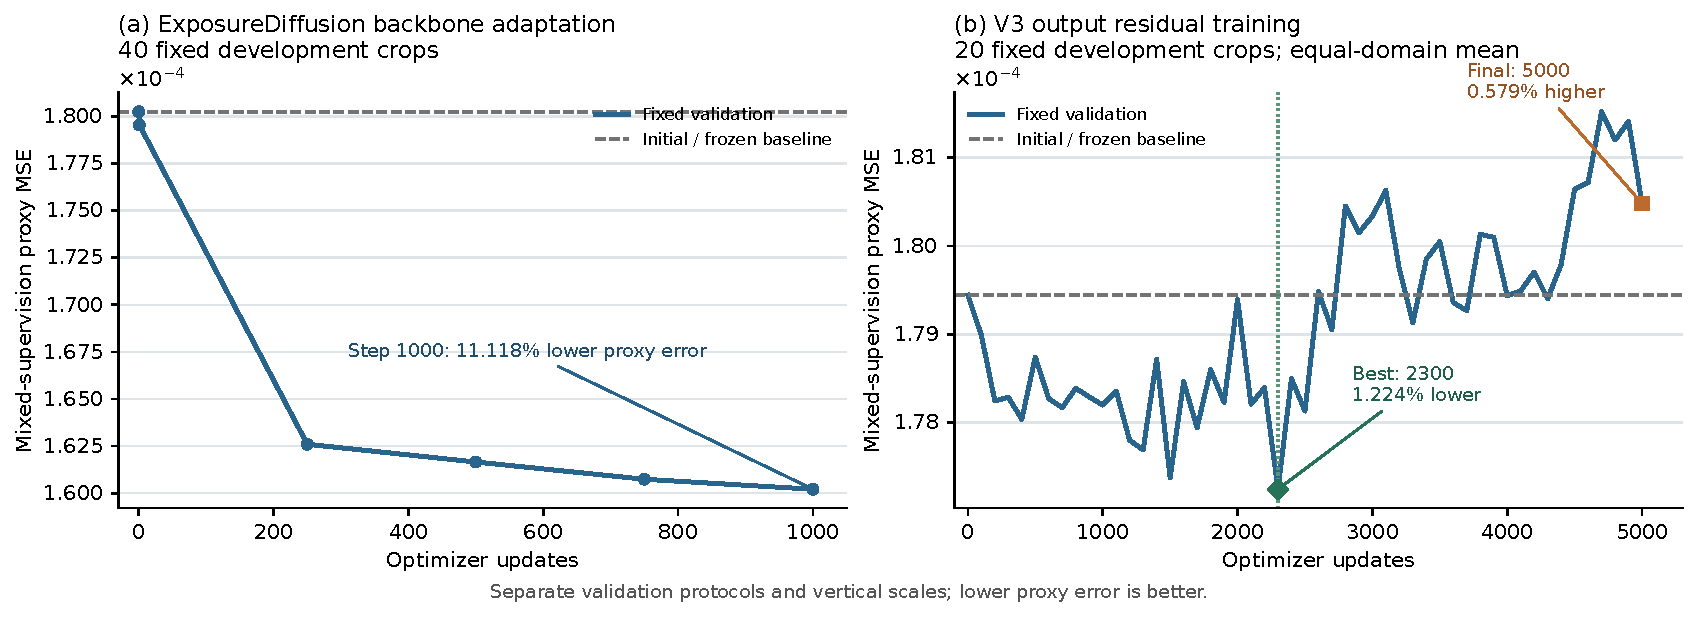
\includegraphics[width=\textwidth]{djc/djc_training_curves.pdf}
\caption{单帧适配和五帧输出补偿的固定验证曲线。左图是单帧阶段的40个裁块，右图是五帧阶段的20个裁块、按开发域等权汇总。两图都只比较训练前后的代理误差，绝对值不能直接比，下降比例也不能相加。五帧候选在第2300步最好，继续训到5000步反而比冻结基线还高。}
\label{fig:djc_training}
\end{figure}

如图\ref{fig:djc_training}，五帧阶段的冻结基线是$1.794418\times10^{-4}$，第2300步降到$1.772457\times10^{-4}$，降了1.224\%；第5000步又升回$1.804805\times10^{-4}$，比基线还高0.579\%。所以在做额外测试之前，我们就定了第2300步为这条线的候选，第5000步只当作训练终点对照。它和单帧适配那11.118\%用的不是同一套验证设置，两个数不能拼成一个总改善比例。

\begin{figure}[!htbp]
\centering
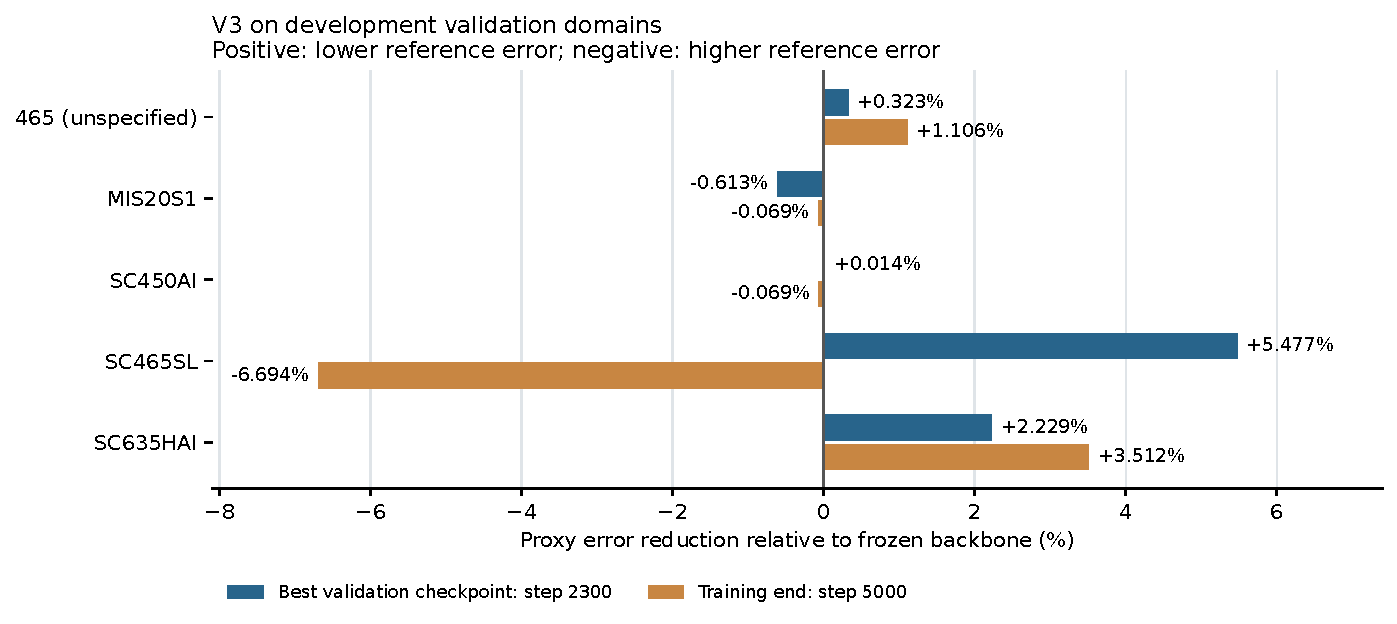
\includegraphics[width=0.94\textwidth]{djc/djc_domain_results.pdf}
\caption{五帧候选的分域固定验证。正值表示代理误差相对冻结单帧基准下降。所有域都出现在开发训练里，属于同域的时间留出；10条型号未确认的465流单独统计。改善随数据域和训练阶段变化，没有哪个域的优势能一直保持。}
\label{fig:djc_domains}
\end{figure}

图\ref{fig:djc_domains}的分域结果，正好说明了总体数字为什么撑不起“采用”两个字。第2300步在 SC465SL 和 SC635HAI 分别下降5.477\%和2.229\%，MIS20S1 反而增加0.613\%；到第5000步，SC465SL 又变成增加6.694\%。回头查固定裁块才发现，SC465SL 有一个裁块只有2个有效运动位置，SC635HAI 有一个只有1个。静态和运动误差是分别归一化的，这么少的位置照样占0.5倍运动项的权重，代理误差自然对局部的教师目标很敏感。这里的位置指 packed Bayer 空间位置，损失在四个通道上计算。

补充实验在同样的开发视频里另取两组20个裁块：第2300步分别改善0.352\%和0.931\%，第5000步反而改善0.807\%和2.283\%。这只是换了裁块位置的随机种子，不是新数据集，也不是独立重复训练，我们也没有据此重新选权重。邻帧诊断里，第2300步把真实五帧换成重复中心帧，输出差异 RMS 的中位数只有0.0134\dn；反转邻帧顺序是0.00834\dn；而残差 RMS 的中位数是0.880\dn。这三项都先在显示 ISP 之前的12位 DN 域按裁块算 RMS，再取20个裁块的中位数。合起来看，候选确有一点统计上的收益，但排序受裁块构成影响，最好的候选对邻帧的利用也很弱，结构有没有改善还得回到画面上去判断。

\subsection{从实际画面决定是否采用}

最后整理出来的是27条场景流、165个同帧案例：20条开发流各3帧，共60例；7条暗房留出流各15帧，共105例。每一例都保留输入、公开预训练基线、公司单帧基准、第2300步候选和第5000步终点。全图和局部面板是同一个案例的两种展示，不另算样本数。下面四列都按流固定了白平衡和亮度映射，展示参数取自该流第一个展示输入帧。这些画面没有干净真值。

\begin{figure}[!htbp]
\centering\small
\djchead
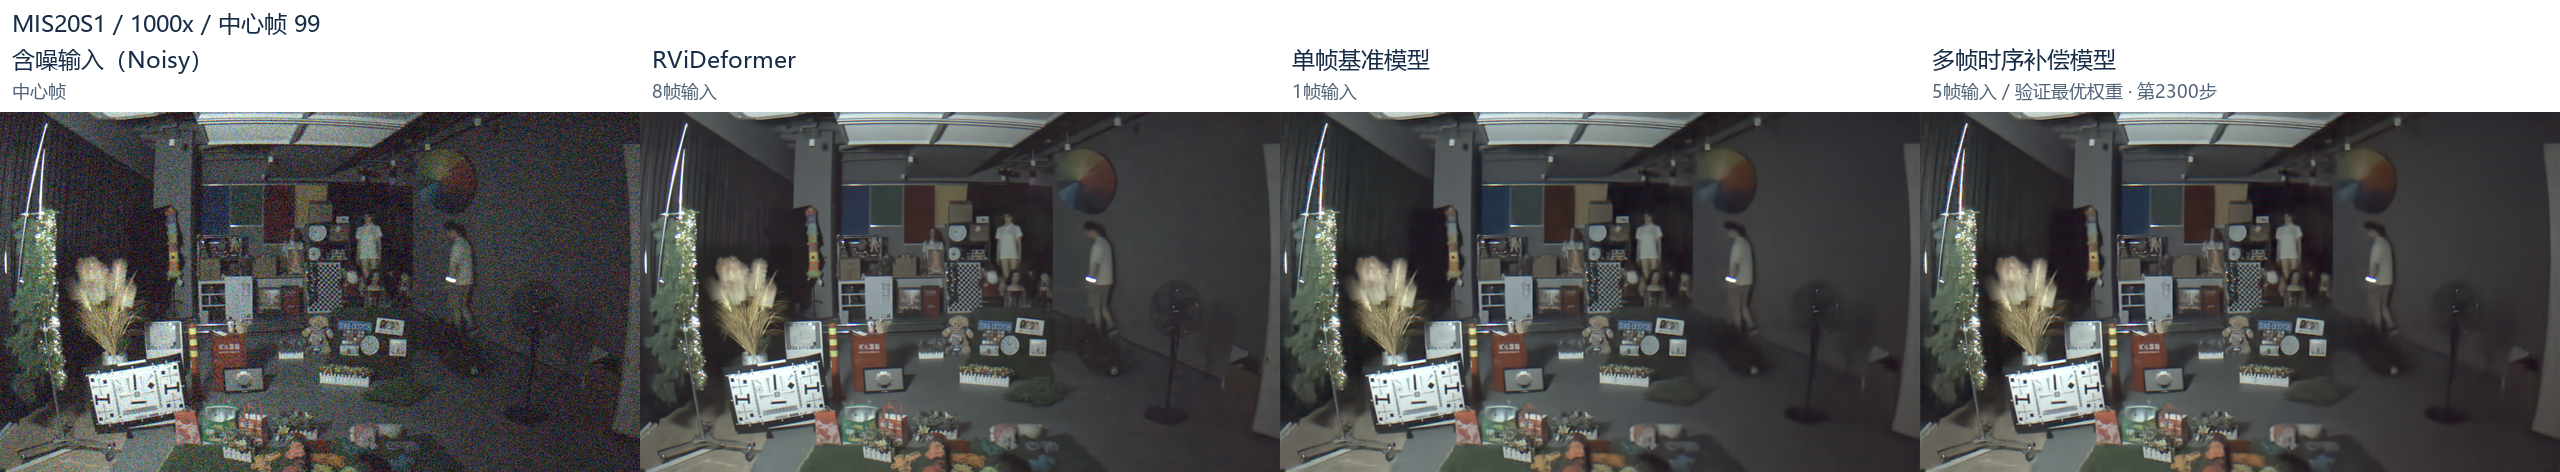
\includegraphics[width=\textwidth,trim=0 0 0 112bp,clip]{djc/djc_1000x_full.png}\\[0.35em]
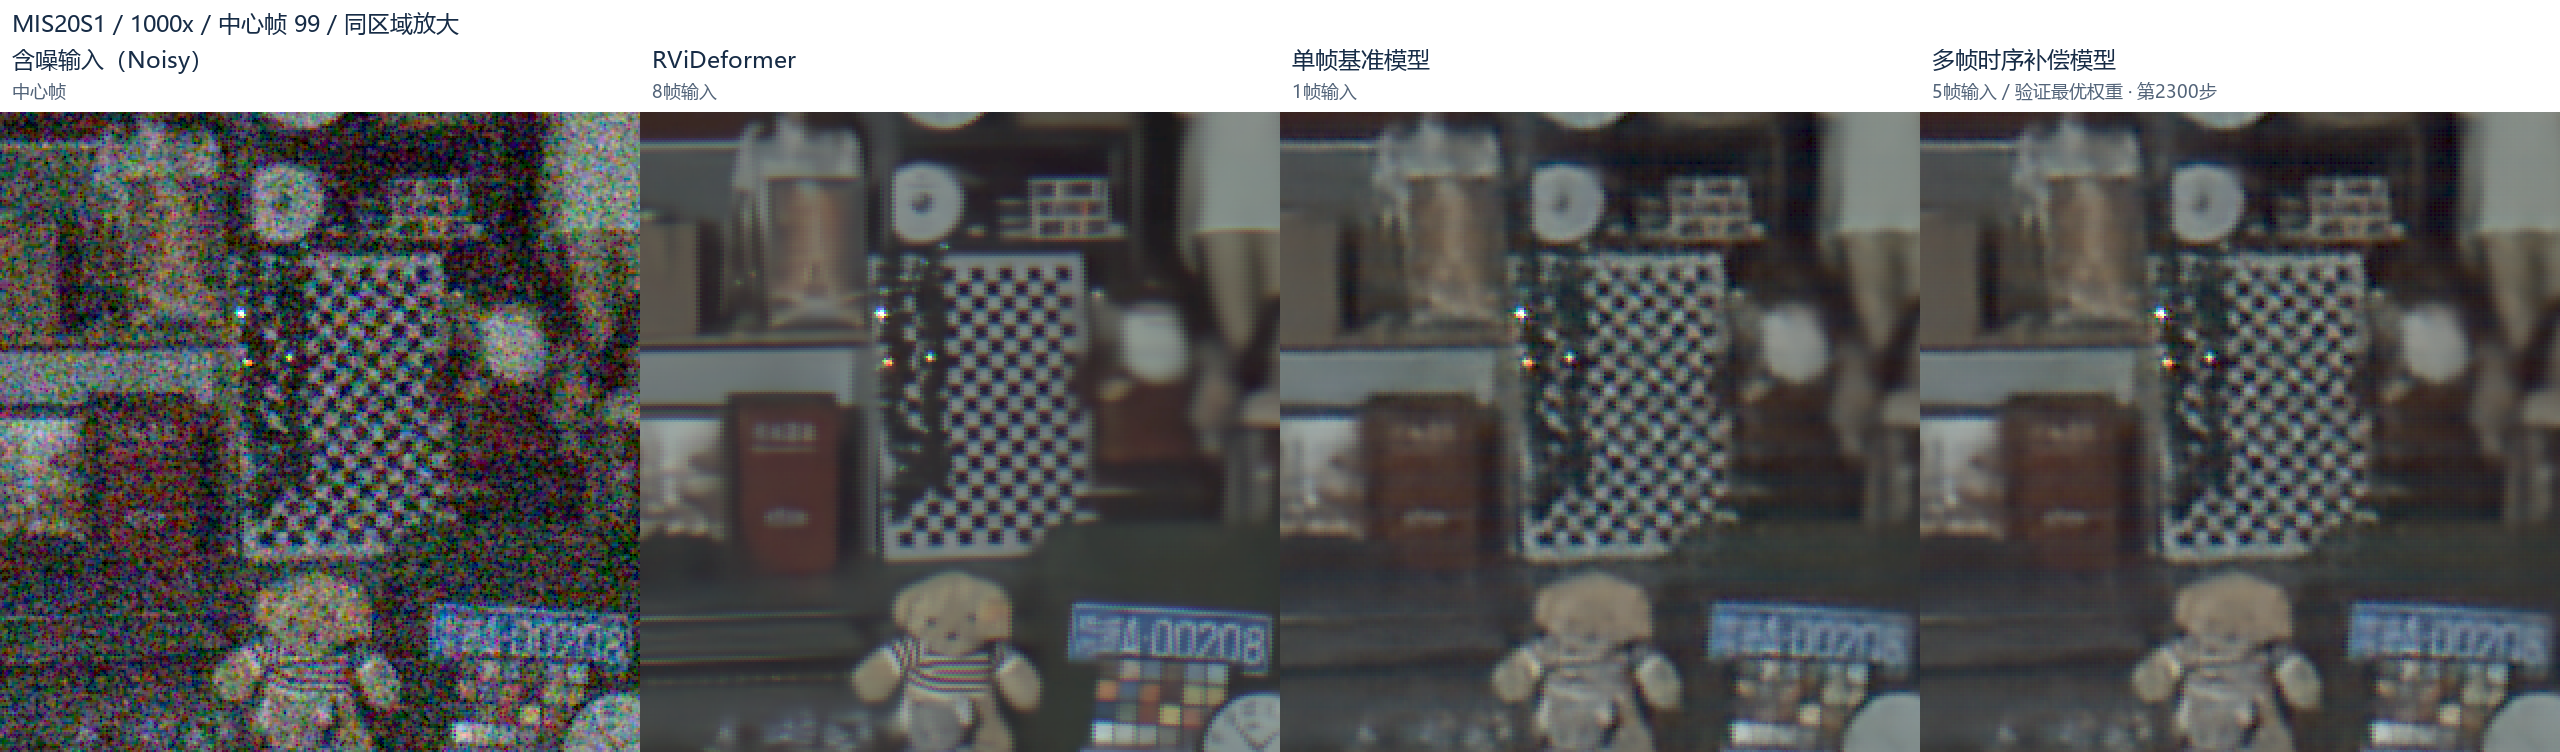
\includegraphics[width=\textwidth,trim=0 0 0 112bp,clip]{djc/djc_1000x_detail.png}
\caption{MIS20S1 暗房1000x序列第99帧，全图和同位置局部。这条序列没有参加本线的训练和选权重。四列依次是输入、使用 CRVD 权重的八帧公开预训练基线、公司单帧基准、五帧输出补偿第2300步。后两列总体上很接近，棋盘格和玩偶衣服的条纹在公开预训练基线的输出里更好认。这里的公开预训练基线是冻结参照，不是后文方法3的后训练权重。}
\label{fig:djc_1000}
\end{figure}

图\ref{fig:djc_1000}是这条线最直接的取舍依据。单帧适配和残差补偿都能把噪声压下去，但在高噪声的图卡和玩偶区域，五帧候选基本贴着单帧基准，看不出足够明确的细节恢复。公开预训练基线自己也有平滑问题，在这个样本上却保住了更可辨的结构。这组对照不是等参数、等帧数的消融，它回答的是很实际的问题：当前候选能不能换掉现有的视频教师。

\begin{figure}[!htbp]
\centering\small
\djchead
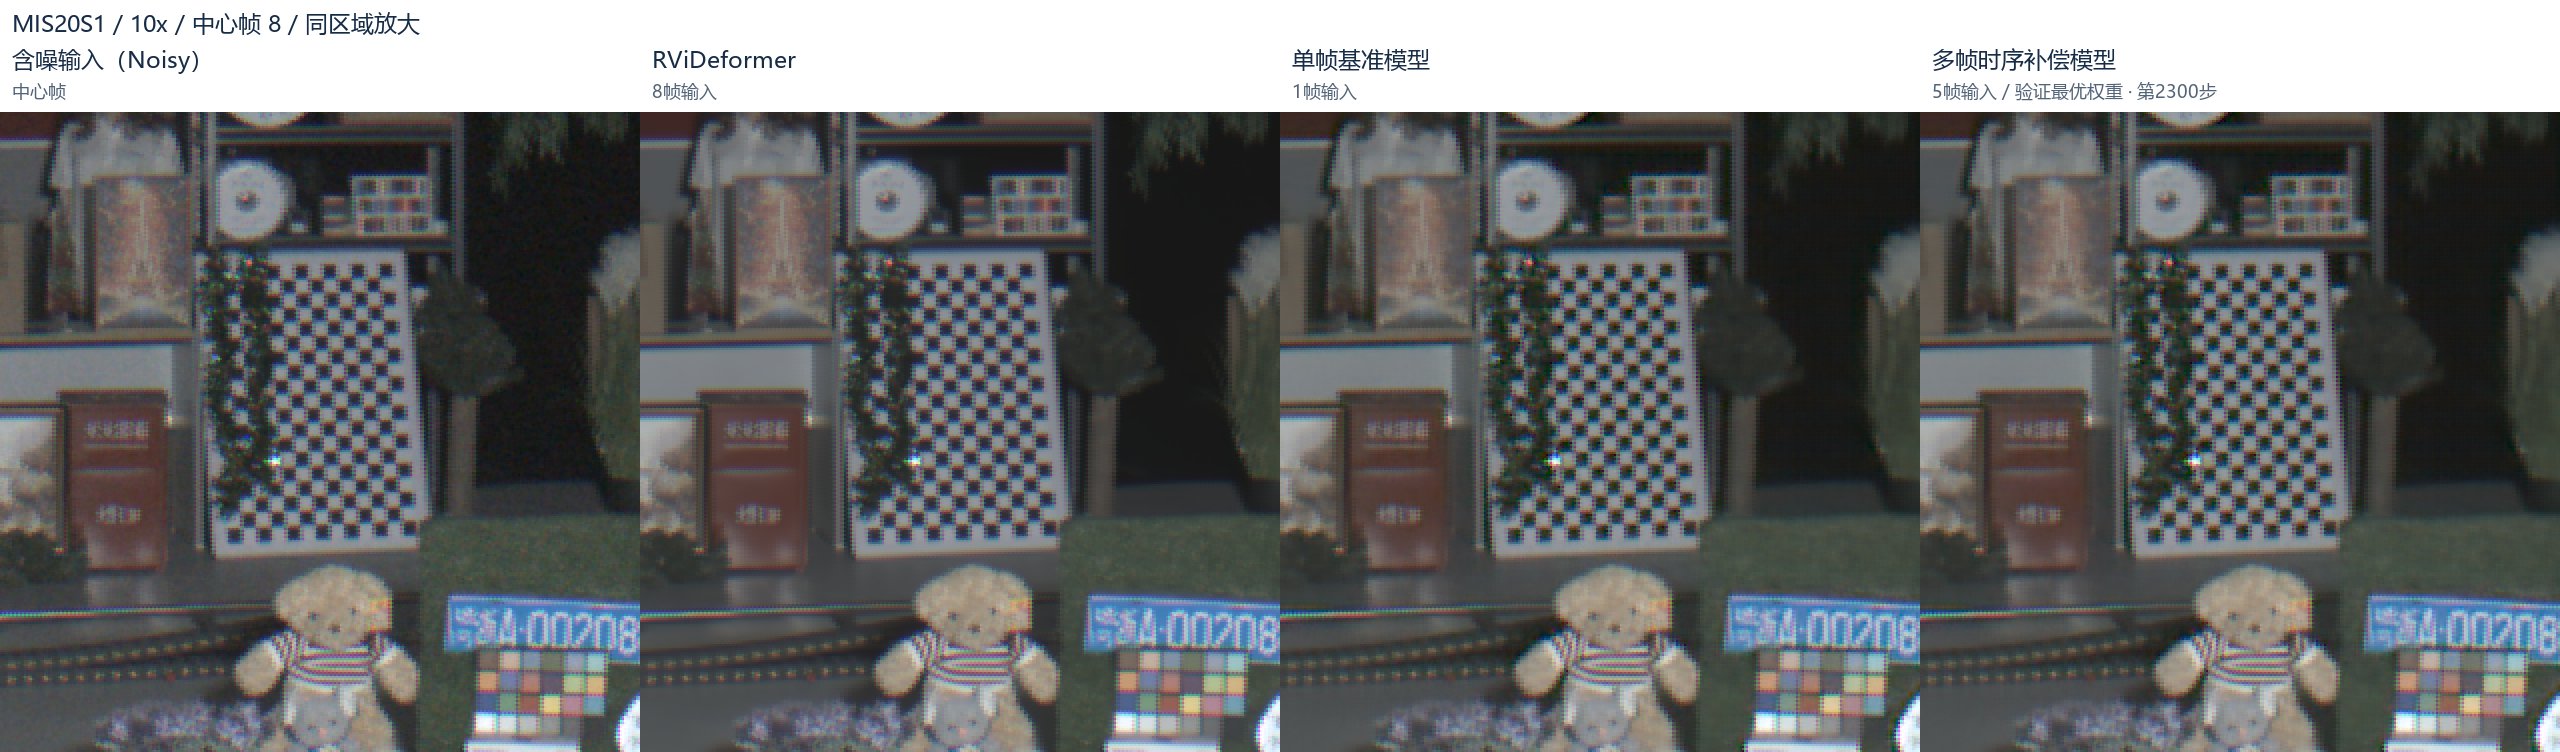
\includegraphics[width=\textwidth,trim=0 0 0 112bp,clip]{djc/djc_10x_detail.png}
\caption{MIS20S1 暗房10x序列第8帧，列的顺序同图\ref{fig:djc_1000}。这条流同样在本线留出。低噪输入本身结构就比较清楚，几个模型之间的差异比1000x样本小，五帧补偿仍然没有普遍的、看得清的细节增益。到方法3里这条流会被用来构建参考，同一条数据在不同路线上的身份是分开记的。}
\label{fig:djc_10}
\end{figure}

低噪的留出样本和开发域尾段，是用来查上面这个判断会不会只是被最难样本带偏的。图\ref{fig:djc_10}里差别整体很小；图\ref{fig:djc_sensors}里，SC450AI 的人物和 SC635HAI 的图卡上，五帧输出也还是贴着单帧基准。分域代理误差降了，不等于每个局部都有看得见的收益。这批静帧更说明不了连续视频里的闪烁或重影有没有改善。

\begin{figure}[!htbp]
\centering\small
\djchead
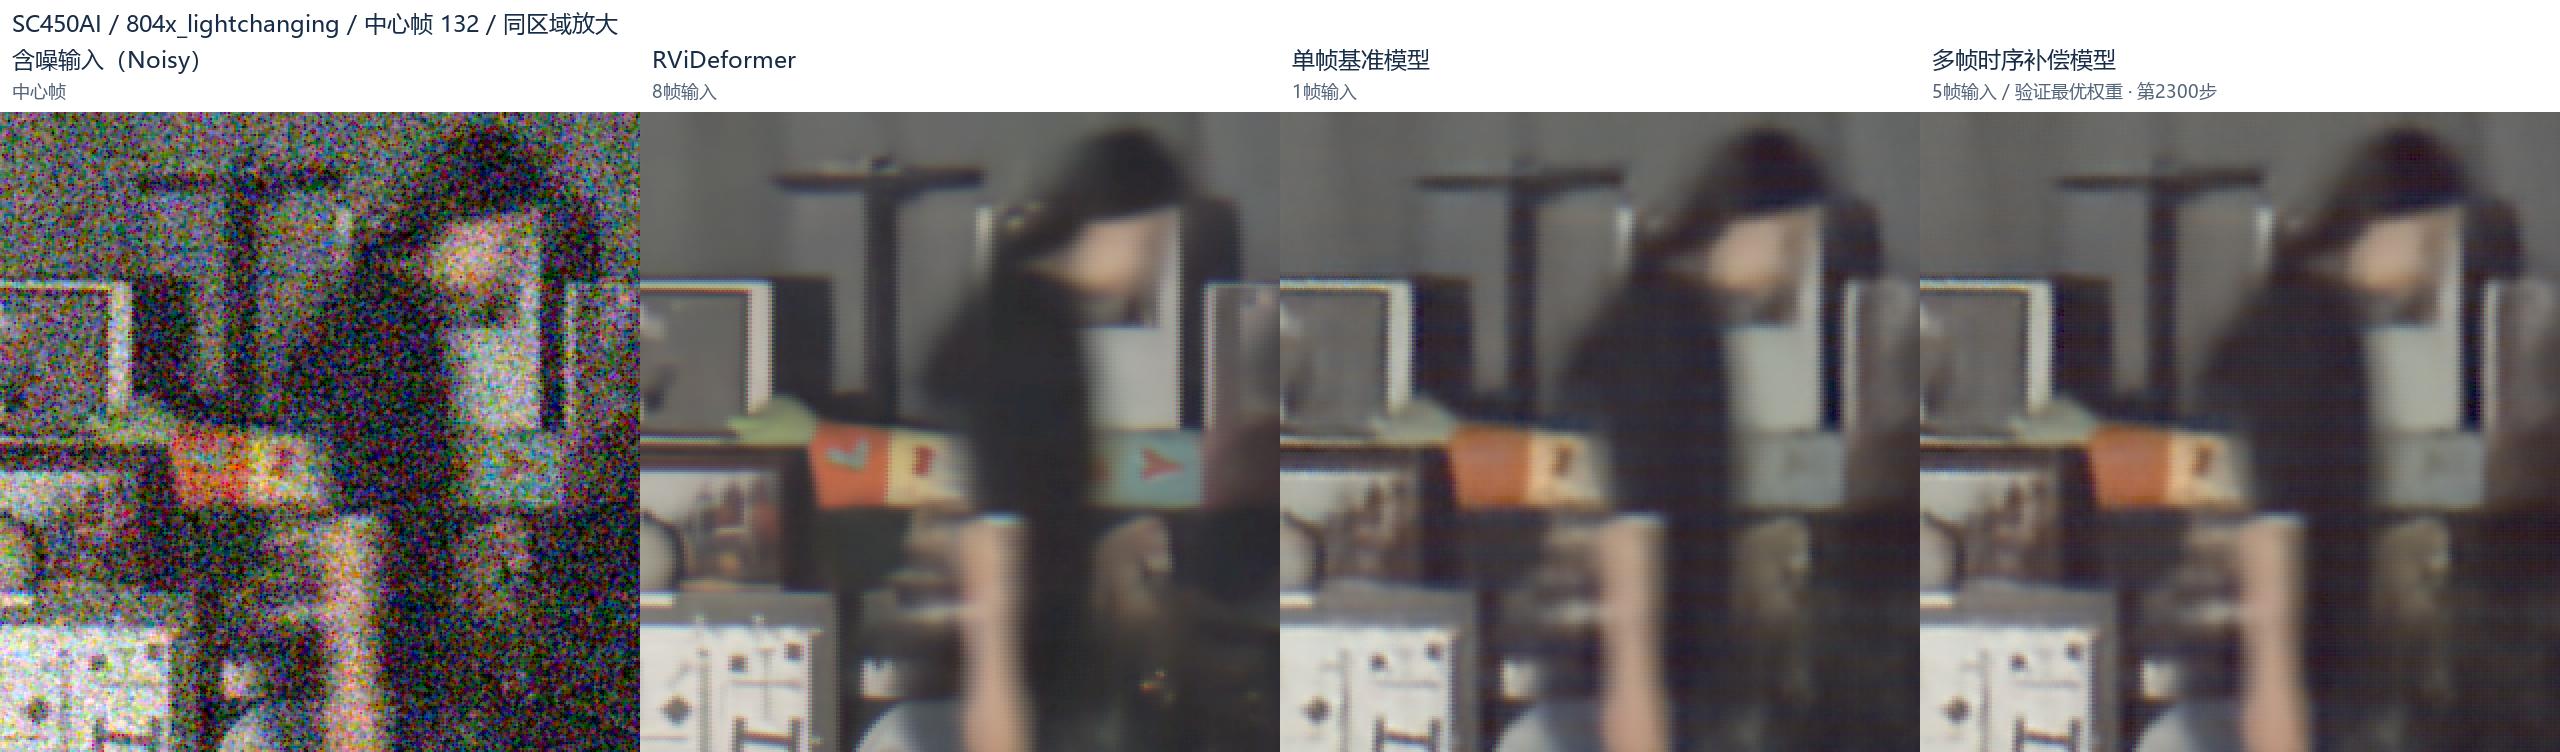
\includegraphics[width=\textwidth,trim=0 0 0 112bp,clip]{djc/djc_sc450_detail.png}\\[0.4em]
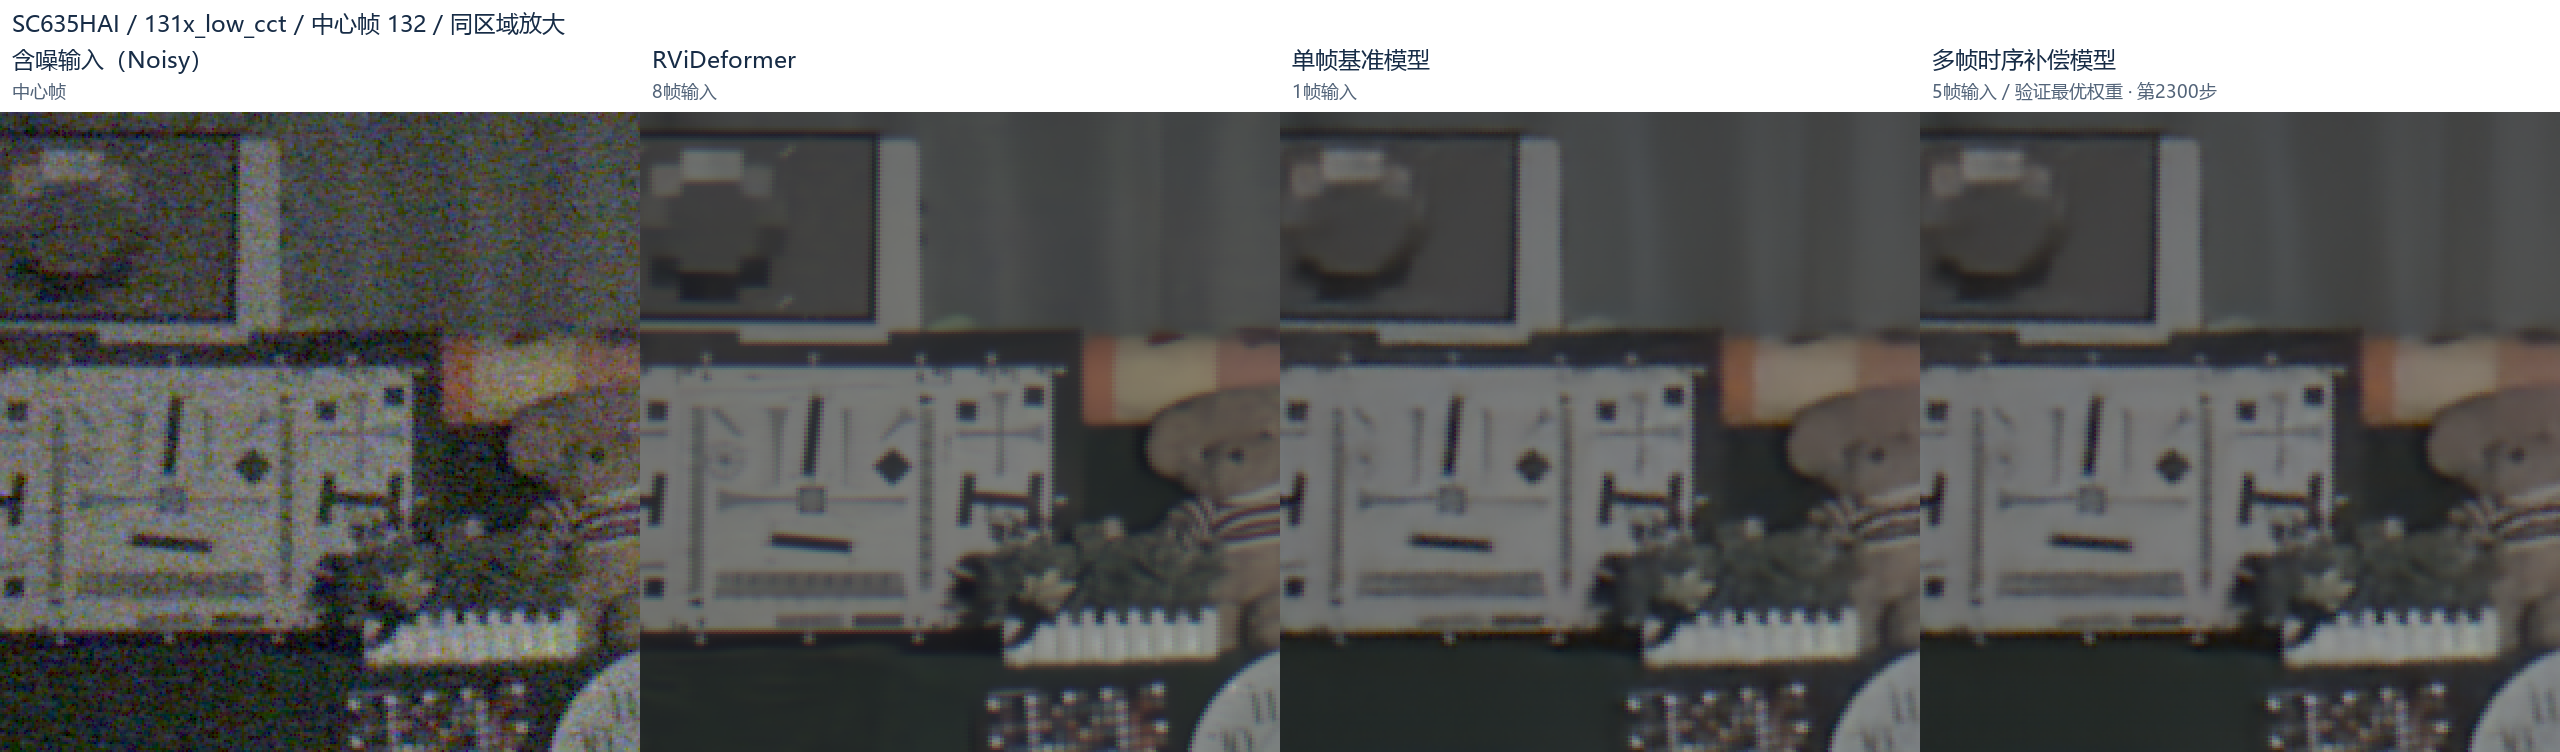
\includegraphics[width=\textwidth,trim=0 0 0 112bp,clip]{djc/djc_sc635_detail.png}
\caption{开发域的时间留出画面：上图是 SC450AI 灯光变化804x序列第132帧，下图是 SC635HAI 低色温131x序列第132帧。四列不变，还是输入、公开预训练基线、单帧基准和五帧第2300步候选。两条流的前段参与了训练，图示的尾段属于验证，不能叫新传感器零样本结果。}
\label{fig:djc_sensors}
\end{figure}

\subsection{未采纳的原因与时空联合恢复的动机}

公司单帧适配确实把原来的固定代理误差降了下来，后面的补偿和解冻实验也都有可测的收益。但我们要的不是一个指标好看一点，而是能稳定替换现有教师的 RAW 视频恢复模型。信息接入位置、监督方式、更新范围都换着试过，五帧候选的总增益依旧很小，还会随数据和裁块位置摆动，真实的图卡与纹理上始终没有建立起稳定优势。所以在现有数据和已完成的实验范围内，这条改造路线达不到采用要求，最终没有成为 Stage2 的默认方案。

这些结果说明，在当前数据和监督条件下，仅增加外围补偿模块还不足以稳定利用邻帧恢复结构；实际对照中的视频预训练基线则表现出可用的时空表征。因此，后续方案把跨帧融合放在恢复主干内部，并让空间上下文、邻帧信息和细节重建共同参与优化。另一方面，预训练基线本身仍会平滑公司数据中的高频内容，说明网络的聚合能力还需要适合公司域的监督来引导。下面先介绍 STaR-RAW 的网络与训练思路，再展开公司域后训练的各项尝试。

\section{STaR-RAW方案与网络架构}
\label{sec:star_method}

\subsection{从补偿探索到时空联合恢复}

我们提出的 STaR-RAW 方案围绕三个相互关联的问题组织：网络如何从含噪视频中利用结构信息，缺少配对干净真值时如何获得训练基础，以及如何将这种基础转化为公司传感器上的恢复能力。前期探索表明，代理误差下降并不必然带来细节改善，因此方案同时关注时空信息的聚合方式与监督对结构保留的约束。

\textbf{让邻帧在主干内部参与恢复。}单帧输入中的弱纹理可能被噪声掩盖，相邻帧则提供同一内容的重复观测。采用端到端的时空恢复主干，可以让跨帧信息在多个特征层级参与重建，而不是只在最终输出上叠加残差。帧间对应由注意力建立，并与当前帧的空间特征共同更新。

\textbf{兼顾局部细节与较远范围的结构。}局部窗口适合保留细线和边缘，但对较大位移及远距离相似内容的利用有限。方案采用多尺度主干与多分支注意力，在局部、低分辨率以及较大邻域之间聚合信息。缩略特征提供较稳定的轮廓线索，原分辨率特征保留细节，两者共同参与后续重建。

\textbf{用公司域监督约束细节保留。}时空平均可以降低噪声，也可能抹去运动和高频结构。为此，后训练只在可信静态区域构造重建目标，结合实测噪声扩充退化条件，并以梯度和高通损失补充像素重建约束。网络、监督与噪声建模共同组成完整方案，运动保真和跨传感器能力则通过后续专项实验检验。

\subsection{网络架构与数据流}
\label{sec:network_flow}

STaR-RAW 采用多分支时空注意力恢复主干，由浅层特征提取、U 形时空重建、全分辨率特征细化和残差输出组成，整体见图\ref{fig:star_raw_overview}。记归一化后的输入为 $X\in\mathbb R^{T\times4\times H\times W}$，其中 $T=8$，$H,W$ 是 packed RAW 的空间尺寸。浅层卷积将每帧4通道映射到84通道，得到 $F_0$；卷积核为 $1\times3\times3$，时间方向不做混合，为后续注意力保留逐帧的空间特征。

\subsubsection{多尺度时空重建}

U 形主干在不同空间尺度上交替聚合时空信息。七个阶段相对 packed RAW 的空间尺度依次为 $1,\,1/2,\,1/4,\,1/8,\,1/4,\,1/2,\,1$，特征宽度均为84，时间长度始终保持8帧。降采样让同一大小的特征窗口覆盖更大的输入区域，有利于在强噪声和帧间位移下寻找相关结构；恢复分辨率时，同尺度编码与解码特征逐元素相加，将细尺度边缘与粗尺度上下文结合起来。

每个阶段包含4个注意力块，当前配置中前3个启用两帧互注意力，随后1个进行窗口自注意力更新。空间多尺度与时间交互共同扩大信息利用范围，避免邻帧只在最终输出处提供一个较弱的补偿量。这里的聚合能力是网络的结构基础，其是否能恢复公司数据中的真实细节，仍需由后训练监督和后续实验检验。

\begin{figure}[!htbp]
\centering
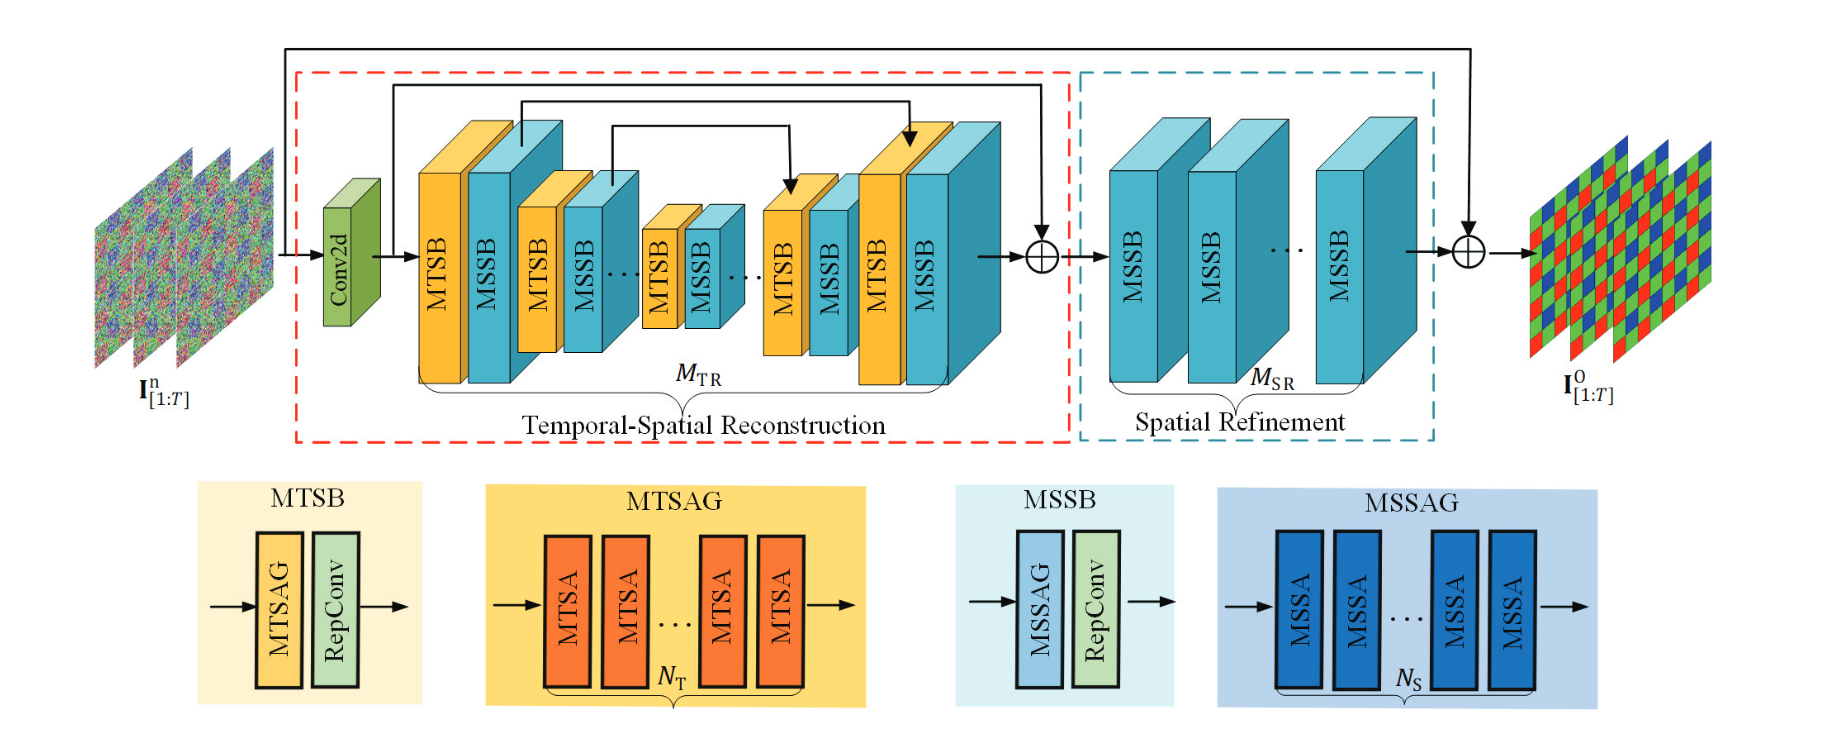
\includegraphics[width=\textwidth]{assets/STaR-RAW/屏幕截图 2026-01-30 151658.png}
\caption{STaR-RAW 所采用的时空恢复主干结构示意。左边是 U 形时空重建，右边是全分辨率特征细化，长跳接用于残差重建。入口的 Conv2d 在本项目中以时间核为1的$1\times3\times3$卷积实现。图中的空间细化模块在本项目配置下仍保留跨帧自注意力。}
\label{fig:star_raw_overview}
\end{figure}

\subsubsection{多分支空间信息聚合}

局部窗口计算量可控，但仅依靠窗口内部的信息，难以利用较远位置的相似结构。图\ref{fig:star_raw_mssa}所示的多分支空间自注意力（MSSA）因此使用相同的查询区域，从不同空间范围提取键和值。忽略位置偏置和移窗掩码时，各分支的基本计算可统一写为
\begin{equation}
 \mathcal A(Q,K,V)=\operatorname{Softmax}\left(\frac{QK^\top}{\sqrt d}\right)V,
 \label{eq:star_attention}
\end{equation}
其中 $d$ 是单个注意力头的特征维度；实际实现还按分支配置加入位置偏置及移窗掩码。注意力权重由特征相似性决定，使输出能够从相关位置聚合信息，而非对窗口内容做无差别平均。

\textbf{局部窗口分支。}查询、键和值均由当前窗口生成，保留局部纹理与边缘之间的细粒度关系。窗口移动后，相邻窗口之间可以交换信息，减少固定窗口划分对结构连续性的限制。

\textbf{低分辨率窗口分支。}查询仍来自当前窗口，键和值来自其空间 $2\times2$ 平均池化版本。空间 token 数降为原来的四分之一，局部随机扰动受到一定抑制，同时保留较稳定的低频轮廓。该分支为强噪声区域提供较平稳的结构线索，与原分辨率分支共同使用，以兼顾噪声抑制和细节保留。

\textbf{较大范围分支。}键和值来自更大邻域或当前特征图的缩略表示。邻域分支扩大搜索范围而不把整张特征图压缩到很小；全局分支则以较少 token 提供更广的上下文。实现按当前特征尺寸选择两者：在本项目 $64\times64$ packed 裁块与 $8\times8$ 空间窗口的配置下，原分辨率使用邻域信息，中低分辨率使用全局缩略信息。三个分支的输出经拼接和线性映射融合。

这里的全局范围是当前输入裁块，而不是未经分块的整幅 RAW。虽然 MSSA 按空间信息来源命名，实际实现采用三维窗口；窗口自注意力可以同时覆盖多帧，不能将所有 MSSA 都理解为独立的逐帧运算。

\subsubsection{跨帧互注意力与隐式对应}

相邻帧对同一结构提供重复观测，但运动会使对应内容偏离相同坐标。多分支时域互注意力（MTSA，图\ref{fig:star_raw_mtsa}）由参考帧窗口生成查询 $Q_r$，由支持帧生成键 $K_s$ 和值 $V_s$，通过 $\mathcal A(Q_r,K_s,V_s)$ 聚合跨帧信息。两帧互换参考与支持角色，形成双向交互。

局部分支在支持帧对应窗口中寻找相关内容，较大范围分支则利用支持帧的邻域或全局缩略特征，缓解运动使内容离开局部窗口的问题。不同范围的互注意力结果与自注意力特征融合，使当前帧结构和邻帧补充信息共同参与恢复。对应关系由注意力隐式建立，本项目主干没有额外启用显式光流对齐模块。

启用互注意力的块使用 $2\times8\times8$ 窗口，随后自注意力块采用配置为 $6\times8\times8$ 的窗口；移窗与多级特征更新逐步交换不同局部时空区域的信息。输入序列长度仍为8帧，局部窗口的时间长度不等于完整输入帧数。扩大跨帧搜索范围提供了利用运动内容的能力，但并不保证动态细节一定得到保留，后文方法5至方法7和方法11继续检验这一问题。

\subsubsection{前馈更新、全分辨率细化与残差输出}

注意力聚合后，前馈层更新通道表示，局部卷积补充邻域建模，残差连接保留输入特征。图中的 RepMLP 使用两条并行线性分支相加后进行激活；RepConv 结合线性映射与局部卷积。本项目保留未融合的训练形式，参数量和推理配置均按实际实现统计。

U 形模块回到全分辨率后，84维特征映射到108维，经过4组细化模块，每组包含2个注意力块，再映射回84维。细化段继续使用可跨帧的窗口自注意力，在输出前进一步协调局部结构与时空特征。若用 $\mathcal U$ 表示 U 形重建、$\mathcal R$ 表示含通道映射的细化过程，整体残差重建可概括为
\begin{equation}
 F_0=\operatorname{Conv}_{\mathrm{in}}(X),\qquad
 \widehat Y=X+\operatorname{Conv}_{\mathrm{out}}\bigl(F_0+\mathcal R(\mathcal U(F_0))\bigr).
 \label{eq:star_reconstruction}
\end{equation}
特征层的长跳接保留浅层信息，RAW 层的跳接让网络学习输入与目标之间的修正量。最终输出仍是8帧、4通道的 packed RAW，不在网络内完成去马赛克或色调映射。具体深度、窗口和7,505,716个可训练参数的配置列于表\ref{tab:model_config}。

\begin{figure}[!t]
\centering
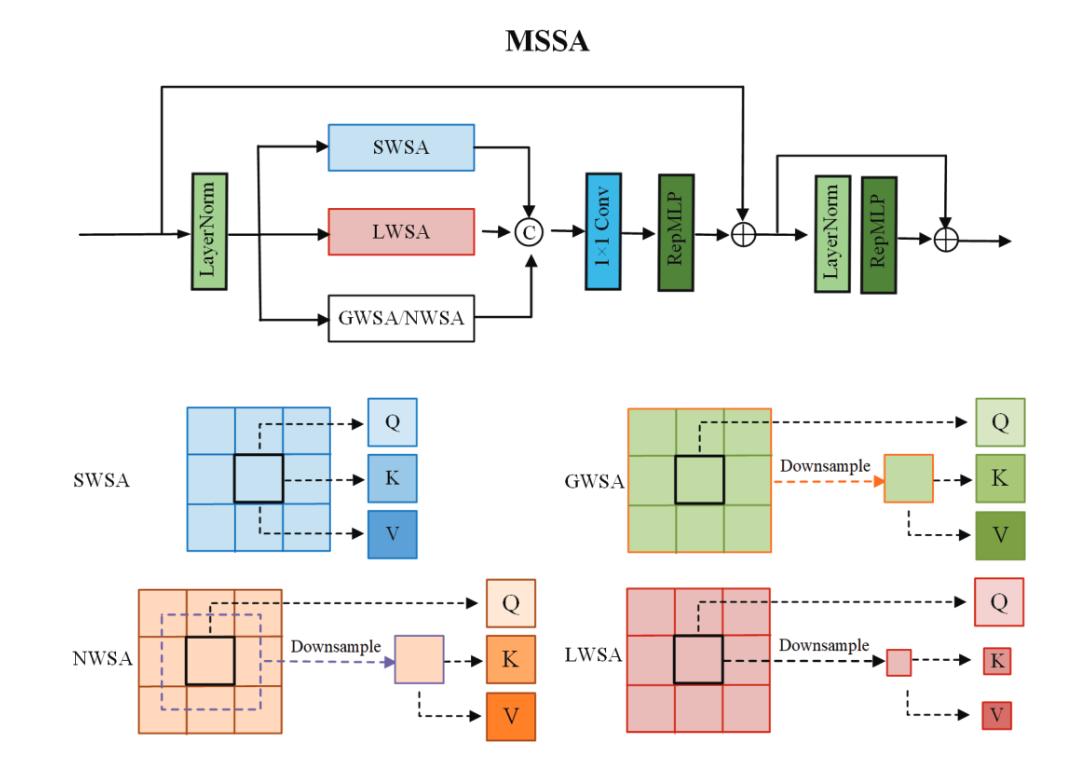
\includegraphics[width=0.80\textwidth]{assets/STaR-RAW/屏幕截图 2026-01-30 183700.png}
\caption{多分支空间自注意力 MSSA 示意。三个分支分别取局部、局部低分辨率和较大范围的信息，后者按特征尺度选用邻域或全局缩略表示。图中 C 表示拼接，圆圈加号表示逐元素相加。}
\label{fig:star_raw_mssa}
\vspace{0.6em}
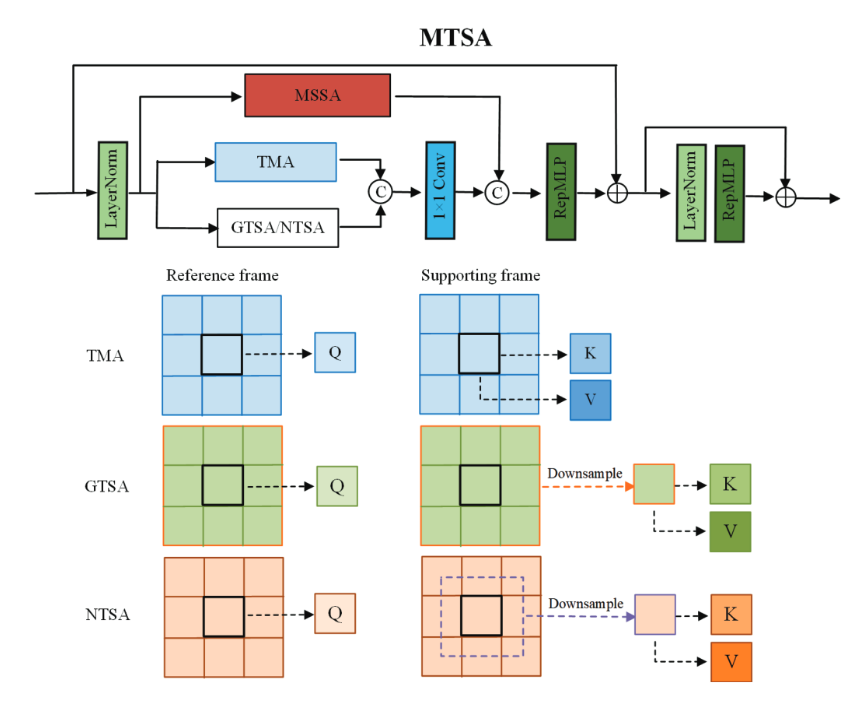
\includegraphics[width=0.80\textwidth]{assets/STaR-RAW/屏幕截图 2026-01-30 204604.png}
\caption{多分支时域互注意力 MTSA 示意。参考帧生成查询，支持帧提供键和值，局部和较大范围的跨帧信息与自注意力特征共同融合。}
\label{fig:star_raw_mtsa}
\end{figure}

\subsection{公开数据预训练基础与公司域迁移}
\label{sec:pretrain_transfer}

公司提供的序列缺少逐帧配对的干净 RAW 真值，难以直接支撑从随机初始化开始的完整视频监督训练。因此，本方案采用公开数据预训练权重作为基础，再从公司静态数据中构建可信参考开展后训练。公开预训练提供基本的噪声抑制和时空表征，公司域后训练则调整模型对目标传感器噪声与细节的处理方式。

本项目使用公开的 CRVD 预训练权重进行初始化。CRVD 数据集\cite{r1}采用逐次静止拍摄、移动物体后再次拍摄的方式构造视频，利用同一静止状态下的多次观测平均获得参考，再按顺序组成含噪与参考视频。室内部分包含11个场景、5档噪声条件，其中6个场景用于训练、5个场景用于测试。这种数据提供了配对监督，但其运动和传感器条件与公司场景仍有差异。预训练权重目录及加载方式列于附录。

公开预训练基线在公司数据上能够降低噪声，但图卡细线、棋盘格、文字边缘等高频结构偏软，部分高增益场景仍有残余噪声。这表明公开数据上的恢复能力尚不能直接满足公司域要求；传感器噪声、量化、固定图样及场景分布的差异，是后续需要检查的因素。我们因此先围绕可构造可靠参考的静态区域建立公司域基线，再扩展到运动和跨传感器测试。

具体而言，低增益长序列提供近似干净的静态参考，同场景不同增益观测提供真实退化样本，平场与黑帧提供可标定的噪声统计。运动、饱和与配准不可靠区域通过掩码排除，避免静态均值把动态内容监督成模糊残影。在此基础上，真实样本与合成样本混合参与后训练，以重建、梯度和高通约束同时优化噪声抑制与结构保留。下面的方法0至方法4构成这一阶段的完整流程。

\section{公司域后训练与后续方案选择}
\label{sec:exploration}

\subsection{方法0至方法4：形成静态基线}

方法0做逐流适配、配准、曝光映射和运动掩码。方法1用暗房10x的200帧构建静态参考，奇偶均值残差0.51--0.80\dn，曝光归一化之后的跨增益偏差1.17--1.86\dn。方法2用平场和黑帧生成9档合成噪声，最大逐通道统计误差8.66\%，在15\%的验收阈值以内。这些准备合起来支撑方法3的混合数据后训练，方法4负责评估。

评测的标准改过一次：1000x 和10x 的跨捕获曝光关系在高亮处偏离线性，同一个模型按这套映射算只有18.84\db。复核配准之后，改用1000x 自身的静态参考，得到53.27\db，奇偶互斥验证是53.10/53.07\db。这件事让我们保留了方法3，也把跨捕获映射的问题和模型本身的误差分开来查。方法3的监督、损失和推理流程统一放在第\ref{sec:adopted}节讲。

\subsection{方法5至方法7：运动保真探索}

静态去噪好起来之后，645x 视频里的运动人物还带着半透明残影。原来的运动审计里，输出在运动区的帧差只剩输入的27\%--32\%。这就是方法5到方法7的由来；比较的时候我们要求运动响应确有改善，同时静态、原生增益和高频指标不能退。

\begin{table}[!htbp]
\centering\small
\caption{三条运动保真路线的设计与结局。}
\label{tab:motion_trials}
\begin{tabular}{P{0.10\textwidth}P{0.30\textwidth}P{0.38\textwidth}P{0.10\textwidth}}
\toprule
方法 & 设计 & 主要结果 & 取舍 \\
\midrule
方法5 & 光流对齐的动态 N2N；教师静态锚；冻结范围与损失权重实验 & 收紧运动置信规则后覆盖仅1.81\%--3.82\%；多组候选未同时通过运动、静态和1000x门槛 & 未采纳 \\
方法6 & 冻结方法3，训练空间残差运动专家；共4版 & 门控 IoU 达0.533，但真实动态内容未稳定恢复；更强残差伴随静态偏移或目标误差增大 & 未采纳 \\
方法7 & 在运动区融合旧教师残差，扫描36组配置 & 最强配置的运动比相对增加0.9162\%；固定 ISP 未见稳定的人物轮廓改善 & 未采纳 \\
\bottomrule
\end{tabular}
\end{table}

方法5用 DIS 光流把后帧对齐到当前帧，靠前向、后向误差和光度误差筛可信像素；加了严格的1像素运动门槛之后，监督覆盖一下就小了。方法6改成冻结主干，减少全模型的漂移；方法7干脆不训练，只检验旧教师的残差能不能直接补上运动信息。三条路依次把参数更新的影响降到零，但在现有数据和验收条件下，都没有拿出足以替换基线的结果。

所以后面的实验仍然保留方法3，重心转到跨传感器：先看同一份权重在哪些数据域上有效，再决定要不要做目标域适配。

\subsection{方法8至方法10：跨传感器适配与退化验证}

零样本测试下来，方法3在 SC465SL 暗室和 sc635hai 低色温的静态域上降噪收益很明显，但 sc450ai 的黑色运动物体还是明显发软。方法8于是试逐传感器适配：sc635hai 用奇偶静态监督，sc450ai 用单帧盲点监督，两边都混入 MIS20S1 回放。最后只留下 sc635hai 的专用输出头，配置见第\ref{sec:head}节；sc450ai 的5个检查点都没能把高频恢复出来，1435x 的端点裁剪反而从3.28\%升到4.64\%。

方法9试的是一次覆盖4种传感器的统一后训练，只更新15,508个参数、训练100步。SC465SL 和 sc635hai 的静态指标略升，sc450ai 的高频比却从0.126621掉到0.126589，黑衣和运动轮廓也没有改善，所以没有当成统一模型采用。

方法10接着查 sc450ai 的监督该从哪来。现有数据只有两条动态场景流，没有独立的暗场、平场，也没有干净的 RAW 配对。补充的退化实验比较了三种噪声：原独立噪声、4\dn{}量化独立噪声和频谱整形噪声。频谱整形把804x 的聚合相关误差改善了，但逐通道噪声和1435x 保留集这两关没过。这个生成器没有进最终方法。

这组实验之后，泛化评测默认用同一份方法3权重，只给 sc635hai 留一个专用可选头；目标域的零样本结果和专用适配结果分开报告。

\subsection{方法11：高增益推理门控}

全数据集预览里，MIS20S1 室外1500x 这类序列还有运动发朦的问题。我们做了四路对比：原始输入、正常时域推理、加权空间拼接、把单帧重复8次的推理。改拼接权重对主体几乎没有影响，单帧重复倒是把更多当前帧的结构带了回来，代价是明显的彩噪。这几组观察说明，时域融合很可能是这个现象的主要来源。

方法11拿输入残差、梯度和光流置信度当门控，在正常时域输出和单帧重复输出之间做融合。两条代表序列上，非零门控的覆盖只有0.487\%和0.713\%，输出整体还是贴着原来的时域分支，逐帧看也没有稳定的主体重影改善，于是没有进最终推理流程。

\subsection{最终方案的确定}

从 ExposureDiffusion 的补偿探索，到 STaR-RAW 的公司域后训练，再到运动和传感器的专项实验，我们逐步区分了代理误差改善、结构恢复与跨传感器泛化。最后保留的方法3具有完整的监督和评测记录，静态恢复也稳定；其余作为默认替代的候选，都没有在各自的目标上达到采用条件。方法8的 sc635hai 输出头以专用可选权重单独保留。下面讲这两项的最终实现，效果统一放到多数据集测试里看。

\section{最终采纳的方法}
\label{sec:adopted}

\subsection{整体流程}

STaR-RAW 在公开预训练基础上，通过 RAW 适配、可信静态监督、真实样本与合成样本的混合后训练、EMA 多帧推理形成公司域恢复流程。方法0到方法2里的数据处理和监督构造，本身就是方法3完整后训练管线的一部分。

\begin{figure}[!htbp]
\centering\small
\fbox{\parbox[c][1.5cm][c]{0.25\textwidth}{\centering 原始 RAW\\位对齐、CFA、黑电平\\配准与曝光映射}}
$\longrightarrow$
\fbox{\parbox[c][1.5cm][c]{0.25\textwidth}{\centering 静态参考与有效掩码\\实测噪声合成\\真实:合成约1:1}}
$\longrightarrow$
\fbox{\parbox[c][1.5cm][c]{0.25\textwidth}{\centering STaR-RAW\\全参数后训练5000步\\EMA权重推理}}
\caption{方法3的完整流程。训练数据统一进到参考域；输出按各自协议在参考 DN 域评测，再用该协议的固定 ISP 展示。}
\label{fig:adopted_pipeline}
\end{figure}

模型输入是8帧、4通道的 packed Bayer，输出是对应的8帧。训练用 $64\times64$ 的 packed patch，对应原 Bayer 的 $128\times128$ 区域；推理则靠重叠分块把整幅画面跑完。方法3没有加增益标签输入，也没有传感器条件分支。

\subsection{真实样本与静态监督构建}

主参考是 MIS20S1 暗房10x 序列200帧的平均。构建时做了固定图样修正，运动和无效区域也都记了下来。参考的形状是 $4\times540\times960$，奇偶分半残差在 R/Gr/Gb/B 上分别是0.511、0.797、0.763和0.560\dn。图卡的高频检查确认过，平均之后结构还够用。

真实输入用了128x、313x、632x和645x。每个增益的输入先读自身的位置对齐、黑电平和运动记录，再用整数配准和逐通道仿射曝光映射，换到主参考的坐标和亮度域。记映射后的像素为 $x_c$，参考黑电平为 $b_c$，归一化为
\begin{equation}
 \widetilde{x}_c=\operatorname{clip}\left(\frac{x_c-b_c}{4095-b_c},0,1\right).
 \label{eq:normalization}
\end{equation}
目标是同一位置的静态参考，在8个时间位置上重复。

有效掩码要同时满足三条：参考有效、输入8帧都是静态、所有输入通道都没饱和。饱和阈值是映射域的3800\dn，运动掩码阈值0.5。只有这些位置参与损失，免得拿静态均值去要求错位的运动和饱和的内容。1000x 真实序列不进训练。

\subsection{实测噪声合成与混合采样}

合成分支的干净目标还是同一份静态参考，噪声模型由9档平场和黑帧建立。信号相关方差写成
\begin{equation}
 \sigma_c^2(s,G)=a_c\,sG+b_c^{\mathrm{read}}G^2.
\end{equation}
实际生成器保留了每档增益的经验 shot 系数 $\alpha_{c,g}$ 和 read variance $v_{c,g}$，用来对付标定数据里的非单调变化。令 $d$ 为固定图样偏置，$z\sim\mathcal N(0,I)$，$LL^\top=C$ 是聚合通道相关矩阵的 Cholesky 分解，合成就是
\begin{align}
 q &= y+d,\qquad s_c=\max(q_c-b_c,0),\\
 x^{\mathrm{syn}} &= \operatorname{clip}\left(
 \operatorname{round}\left[q+\sqrt{\alpha_g\odot s+v_g}\odot(Lz)\right],0,4095\right).
 \label{eq:synthetic}
\end{align}
实现上用相关高斯采样去匹配信号相关方差。合成完按1\dn{}格点量化，黑电平和合法范围保持原样。

合成增益标签取100、200、400、800、1600、3200、6400、12800和25600，每档生成8个独立的噪声时序变体。8帧的干净内容相同、噪声不同；真实和合成分支按约1:1混合。真实性检验拿合成数据和同档真实数据的高通差分噪声来比，最大逐通道相对误差8.66\%，过了15\%的阈值。逐档参数列在附录。

\subsection{优化目标}

方法3从第\ref{sec:pretrain_transfer}节的公开 CRVD 预训练权重初始化，再进行全参数后训练；网络结构和数据流见第\ref{sec:network_flow}节。

训练时先把预测裁剪到 $[0,1]$，再算带掩码的损失。记
\begin{equation}
 \langle z\rangle_M=\frac{\sum M\odot z}{\max(\sum M,1)},
\end{equation}
其中掩码沿通道维展开。总损失为
\begin{equation}
 \mathcal L=\mathcal L_{\mathrm{char}}+0.1\mathcal L_{\mathrm{grad}}+0.1\mathcal L_{\mathrm{hp}}.
 \label{eq:loss}
\end{equation}
Charbonnier 项\cite{r13}约束重建误差：
\begin{equation}
 \mathcal L_{\mathrm{char}}=\left\langle\sqrt{(\hat y-y)^2+10^{-6}}\right\rangle_M.
\end{equation}
若写为 $\epsilon^2$，则 $\epsilon=10^{-3}$。梯度项约束水平、垂直梯度的幅值差：
\begin{equation}
 \mathcal L_{\mathrm{grad}}=\tfrac12\left(
 \left\langle\left||D_x\hat y|-|D_xy|\right|\right\rangle_{M_x}+
 \left\langle\left||D_y\hat y|-|D_yy|\right|\right\rangle_{M_y}\right),
\end{equation}
其中 $M_x,M_y$ 是相邻有效掩码的乘积。高通项为
\begin{equation}
 H(u)=u-\operatorname{AvgPool}_{3\times3}(u),\qquad
 \mathcal L_{\mathrm{hp}}=\langle|H(\hat y)-H(y)|\rangle_M.
\end{equation}
高通只在空间上算，不跨时间平均。重建项管整体恢复，两个权重0.1的结构项补边缘和局部高频的约束。

\subsection{训练、权重选定与完整画面推理}

方法3用 batch size 1、固定学习率 $10^{-4}$ 的 Adam，FP32，总共5000步。训练是从第200步恢复跑到第5000步的，总步数不额外累加。EMA 衰减0.999，每个优化步都更新。最后固定第5000步的 EMA，后面的探索和多数据集测试都用这份权重当默认模型。

整幅画面推理用8帧时间窗口、时间步长4，空间 tile 是 $64\times64$ packed、步长56。空间和时间上的重叠都等权平均。不足8帧时重复末帧补齐。归一化裁剪之后，再按对应的评测管线恢复 DN 值。分块批大小只管一次并行处理多少 tile，和训练的 batch size 是两回事。

\subsection{sc635hai 专用可选输出头}
\label{sec:head}

方法8在方法3 EMA 的基础上把主干冻住，只更新 \texttt{norm}、\texttt{conv\_after\_body} 和 \texttt{conv\_last} 三处，共6个张量、12,400个参数。这个头由108维 LayerNorm、$108\rightarrow84$ 的线性映射，以及 $84\rightarrow4$、核为 $1\times3\times3$ 的卷积组成。

适配数据是 sc635hai 131x 低色温序列，输入和参考的奇偶帧池互斥。训练时以0.5的概率混入 MIS20S1 回放，压一压原域的漂移。batch size 1，学习率 $10^{-5}$，训500步，BF16 autocast、FP32 损失、EMA 0.999，梯度范数裁剪1.0。500步里 sc635hai 采了238步、回放262步。16x 运动彩色序列原样保留，不参与反向传播。

这个头过了既定的自动检查，登记为 sc635hai 的专用可选权重；统一比较仍然用默认的方法3。下一节把默认权重的零样本结果和专用头的适配结果分开来展示。

\section{多数据集泛化效果展示}
\label{sec:results}

\subsection{展示范围与分组}

这一节看的是方法3在\textbf{公司多数据集、跨传感器、跨拍摄条件}上的泛化。它只在 MIS20S1 暗房的真实样本和对应的合成噪声上训练过；SC465SL、sc635hai、sc450ai 都先拿同一份权重做零样本测试。MIS20S1 室外用来看场景变化，1000x 用来看没参与训练的真实增益。单列的方法8结果只代表 sc635hai 的专用适配。

45条原始流都做了输入与方法3的固定 ISP 对比：每条流取首、中、尾3个连续8帧片段，共24帧，合计1080帧。27条场景流用来看画质，18条标定流用于噪声和数值诊断。45/45 说的是推理覆盖，不是效果统计。下面按数据集给静态指标和代表画面。

\subsection{MIS20S1：训练覆盖增益与未见真实增益}

\begin{table}[!htbp]
\centering\small
\caption{MIS20S1 的静态结果。645x 在训练覆盖范围内，参考是10x 的跨增益参考；1000x 真实序列没参与训练，用原生静态参考。}
\label{tab:mis20s1}
\begin{tabular}{lrrrrrr}
\toprule
协议 & 输入PSNR & 方法3 PSNR & 提升 & 输入RMSE & 方法3 RMSE & HF比 \\
 & (dB) & (dB) & (dB) & (DN) & (DN) & \\
\midrule
645x跨增益参考 & 24.3519 & 29.5729 & +5.2210 & 248.1197 & 136.0228 & 0.9712 \\
1000x原生参考 & 44.6204 & 53.2675 & +8.6471 & 24.0565 & 8.8895 & 0.8562 \\
\bottomrule
\end{tabular}
\end{table}

645x 的噪声降得很明显，高频比0.9712，说明静态图卡的结构和参考比较接近。图\ref{fig:mis645}是同一帧的输入和最终输出：墙面和图卡周围的彩噪少了，棋盘、文字和卡片轮廓还分得开。645x 参与了训练，所以这一行说的是训练域上的恢复效果，不算未见增益的成绩。

\begin{figure}[!htbp]
\centering\pairhead
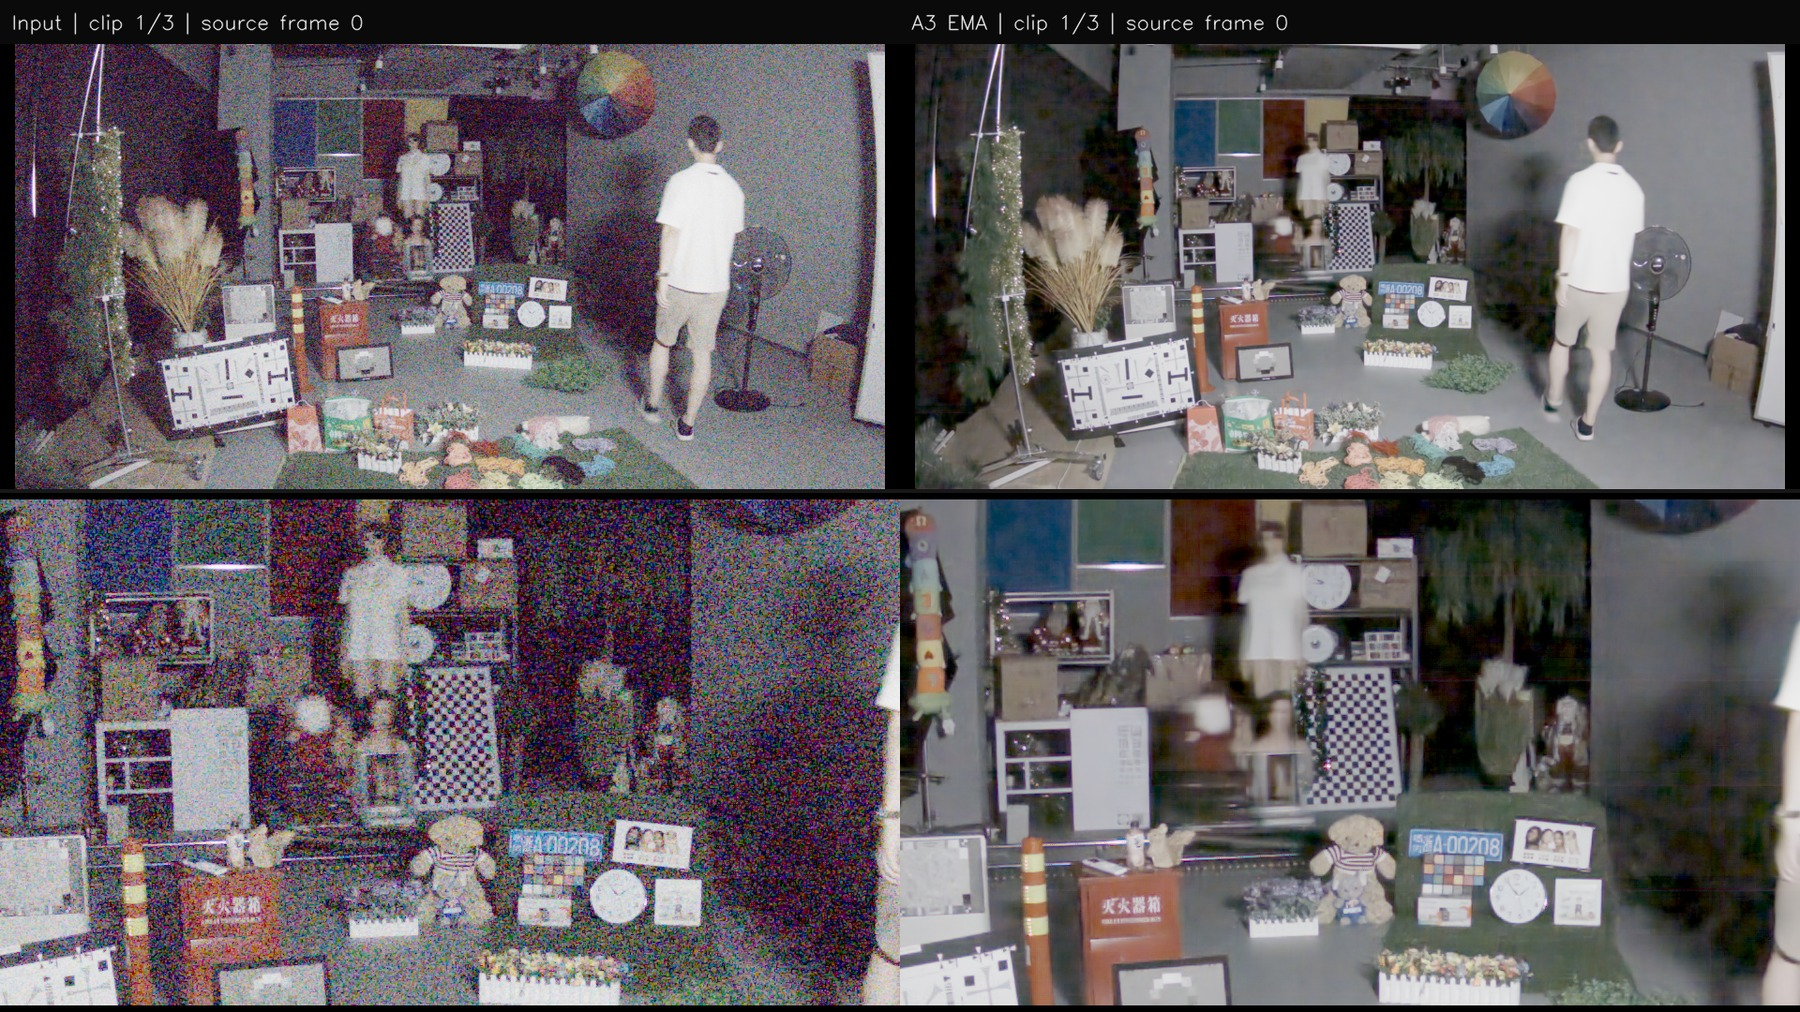
\includegraphics[width=\textwidth,trim=0 0 0 44,clip]{fig04_a3_645x_isp.jpg}
\caption{MIS20S1 暗房645x 的固定 ISP 对比，上为全景，下为固定的中心裁剪。这是方法3在训练覆盖域上的表现，静态定量只统计有效区域。}
\label{fig:mis645}
\end{figure}

1000x 原生参考评测 PSNR 提升8.65\db，RMSE 从24.06\dn{}降到8.89\dn，对应画面在图\ref{fig:mis1000}。为了排除同流参考的影响，我们又用互斥奇偶帧池验了一遍，方法3拿到53.10/53.07\db，和完整原生参考的结果很接近。这说明方法3对没参与训练的1000x 真实流确实有静态去噪能力；不过它仍然是同一间暗房、同一种场景下的真实增益测试。

\begin{figure}[!htbp]
\centering
\makebox[0.32\textwidth]{输入}\hfill\makebox[0.32\textwidth]{方法3（EMA）}\hfill\makebox[0.32\textwidth]{1000x原生参考}\\[0.25em]
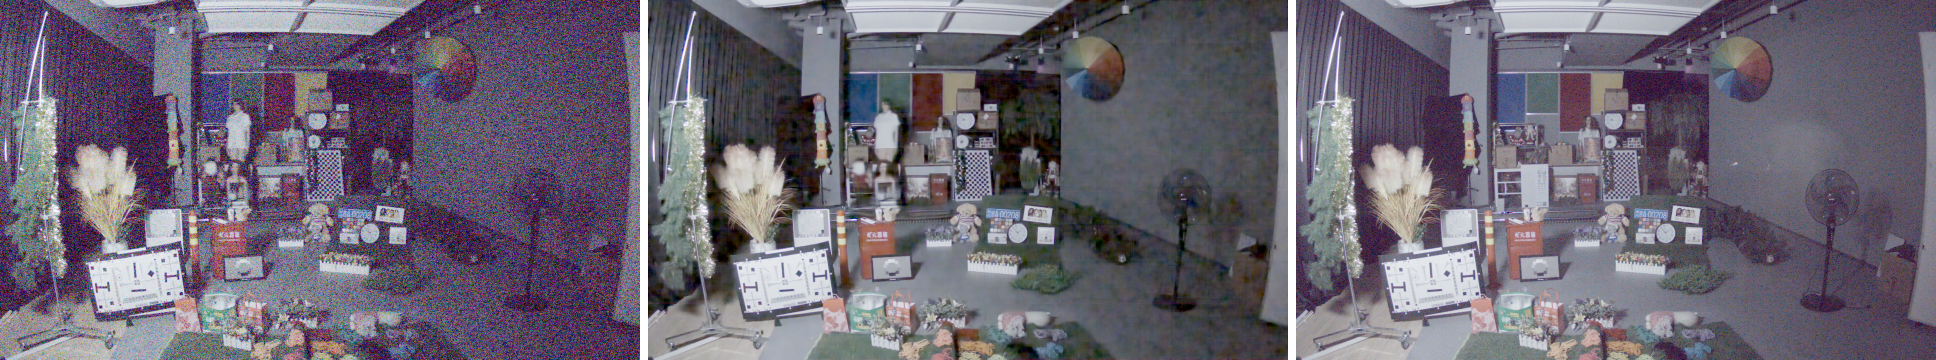
\includegraphics[width=\textwidth]{fig11_native_1000x_traditional_isp.png}
\caption{MIS20S1 1000x 的输入、方法3和原生参考。这条序列不参与主方法训练。展示用的是同一套亮度映射，定量按表\ref{tab:mis20s1}的协议计算。}
\label{fig:mis1000}
\end{figure}

\subsection{SC465SL与sc635hai：跨传感器零样本静态泛化}

表\ref{tab:zero_shot}的结果全部来自同一份方法3 EMA，没有任何目标传感器训练。SC465SL 两档增益提升10.52--13.21\db，sc635hai 低色温静态提升约13.59\db。两个奇偶方向的结果很接近，高频保持率在0.911--0.958之间，输出的 legal RAW fraction 都是100\%。

\begin{table}[H]
\centering\small
\caption{不同数据集上的零样本静态泛化。偶/奇指输入帧池，参考取相反的奇偶池；HF 是输出与参考的高频 RMS 之比，MAD 是时序平均绝对差。}
\label{tab:zero_shot}
\begin{tabular}{llrrrrr}
\toprule
数据集 & 输入池 & 输入PSNR & 方法3 PSNR & 提升 & HF比 & MAD 输入$\to$输出 \\
 & & (dB) & (dB) & (dB) & & (DN) \\
\midrule
SC465SL 256x & 偶 & 41.840 & 55.052 & +13.211 & 0.957 & 31.889$\to$1.567 \\
 & 奇 & 41.840 & 54.999 & +13.158 & 0.958 & 31.886$\to$1.578 \\
SC465SL 2000x & 偶 & 46.039 & 56.563 & +10.523 & 0.911 & 20.238$\to$1.312 \\
 & 奇 & 46.034 & 56.647 & +10.613 & 0.912 & 20.248$\to$1.301 \\
sc635hai 131x & 偶 & 38.737 & 52.325 & +13.588 & 0.919 & 47.481$\to$2.165 \\
 & 奇 & 38.736 & 52.324 & +13.587 & 0.921 & 47.481$\to$2.163 \\
\bottomrule
\end{tabular}
\end{table}

SC465SL 两档的结果分别在图\ref{fig:sc465_256}和图\ref{fig:sc465_2000}。输入里细碎的彩噪和背景波动被压下去了，风扇、人偶、线缆和背景卡片还认得出来。两张图取自完整画面预览，静态定量按各自的有效区域算。图\ref{fig:zero_shot_plot}把三组数据的 PSNR 提升和高频保持率放在一起。

\begin{figure}[H]
\centering
\begin{minipage}{0.90\textwidth}
\centering\pairhead
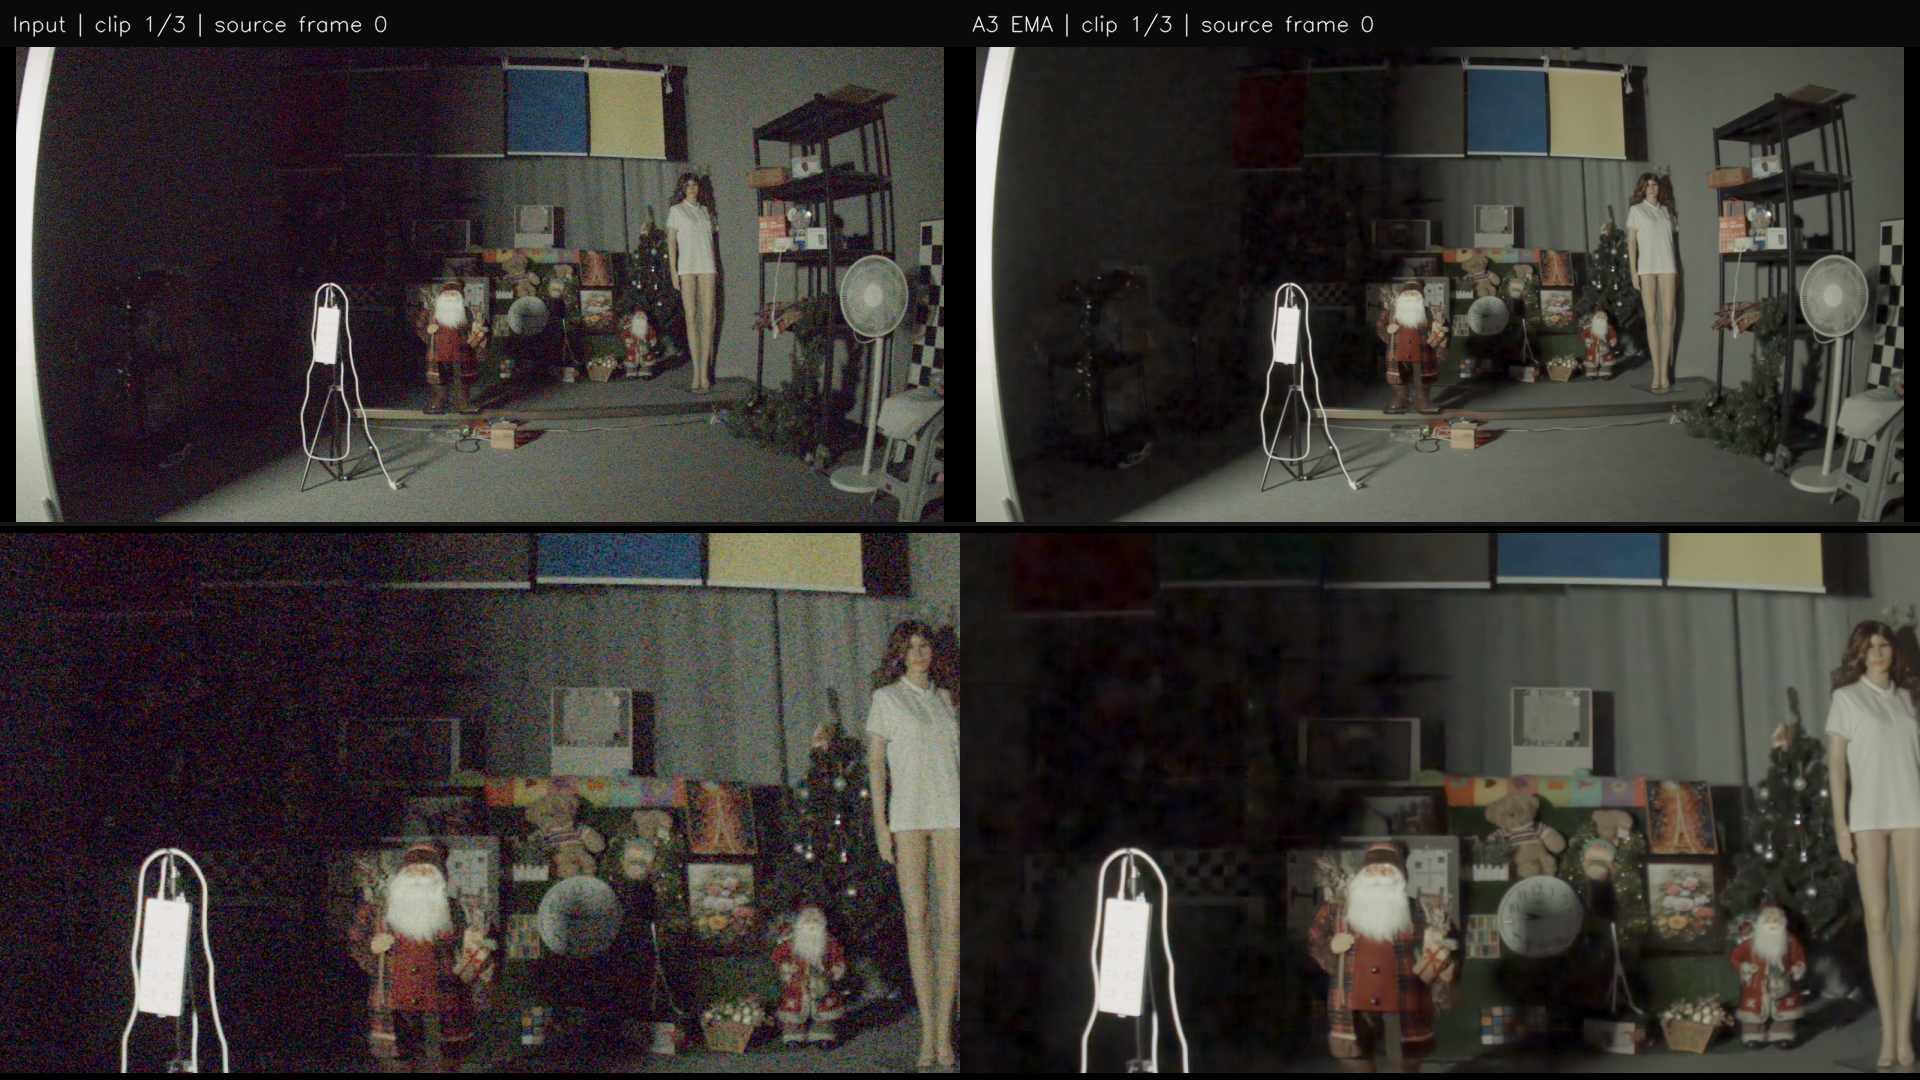
\includegraphics[width=\textwidth,trim=0 0 0 47,clip]{generalization_sc465sl_256x.png}
\caption{SC465SL 暗室256x 的零样本结果，上为全景，下为中心裁剪。模型没在 SC465SL 上训练过。固定 ISP 下噪声明显下降，背景结构也还在。}
\label{fig:sc465_256}
\vspace{0.6em}
\pairhead
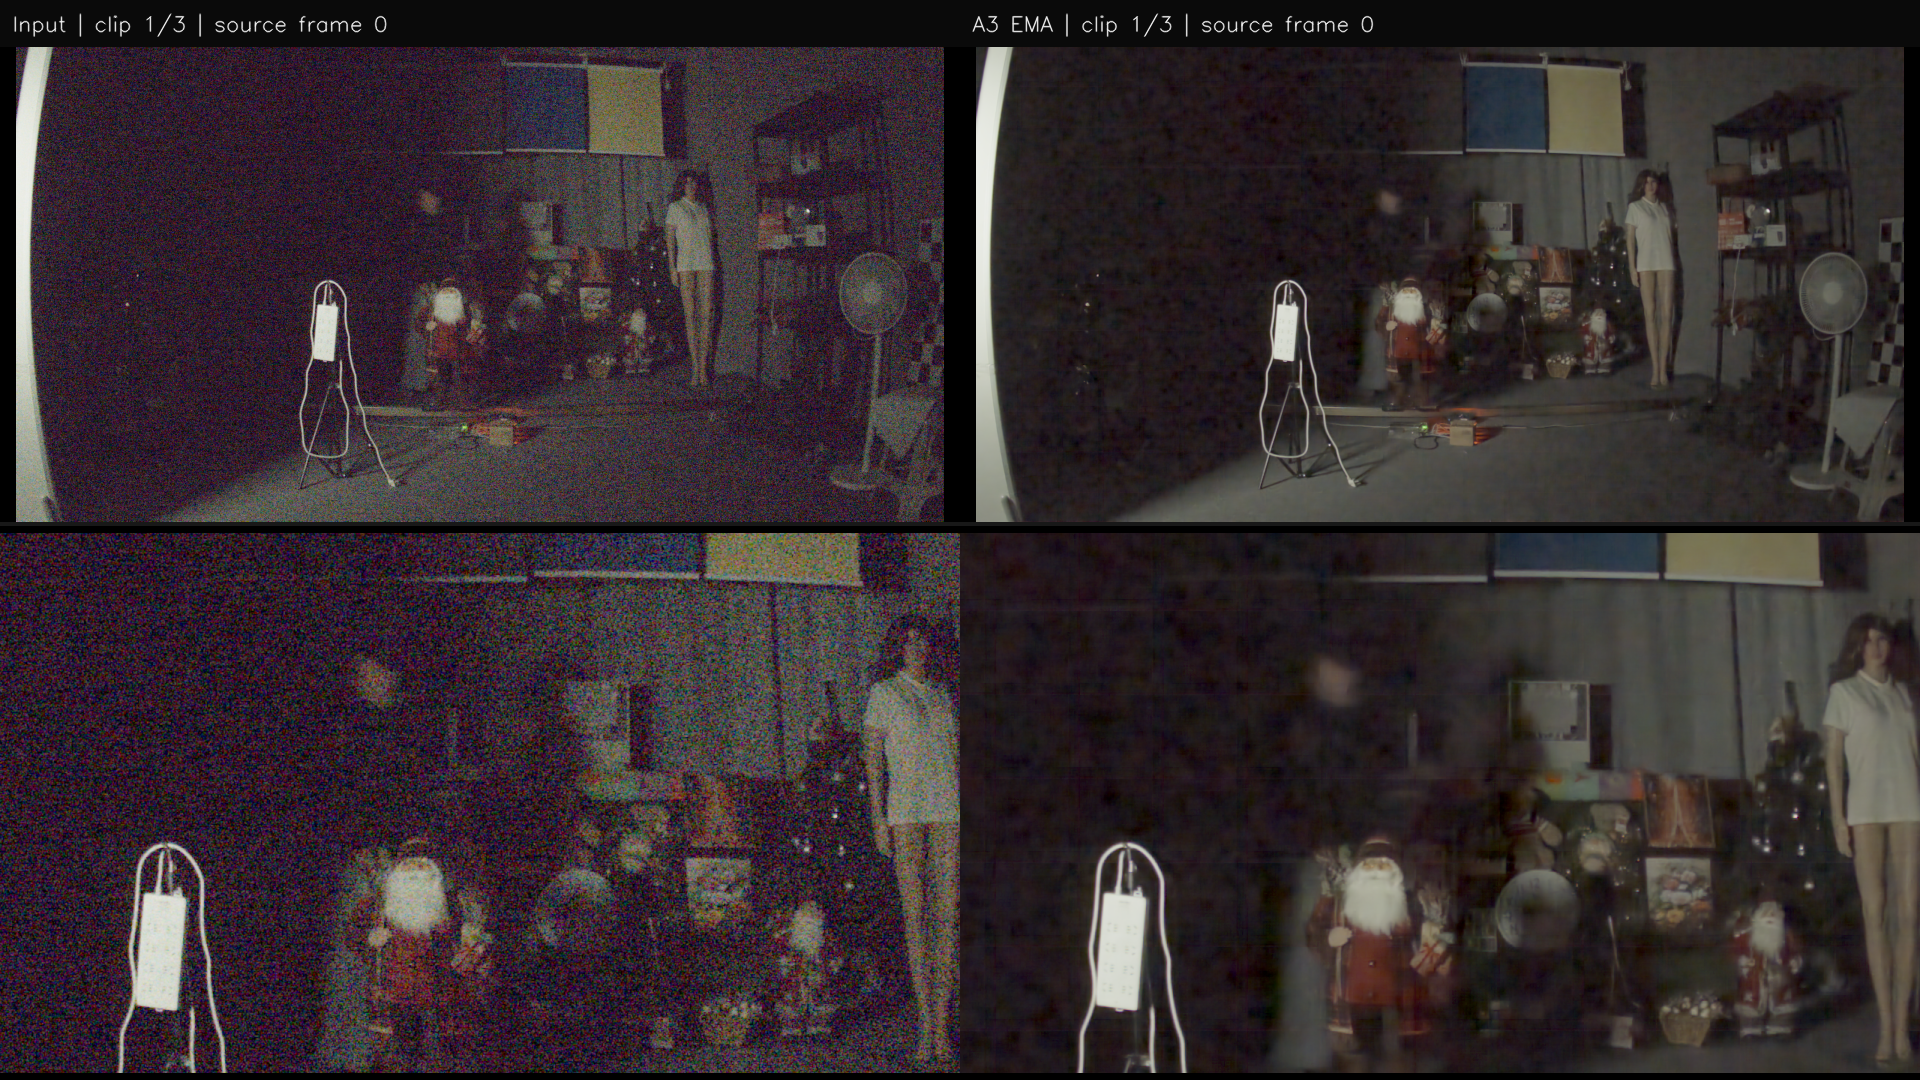
\includegraphics[width=\textwidth,trim=0 0 0 47,clip]{generalization_sc465sl_2000x.png}
\caption{SC465SL 暗室2000x 的零样本结果，权重和推理流程与256x完全相同。静态 PSNR 提升约10.52--10.61\db，高频比约0.911--0.912。}
\label{fig:sc465_2000}
\end{minipage}
\end{figure}

\begin{figure}[H]
\centering
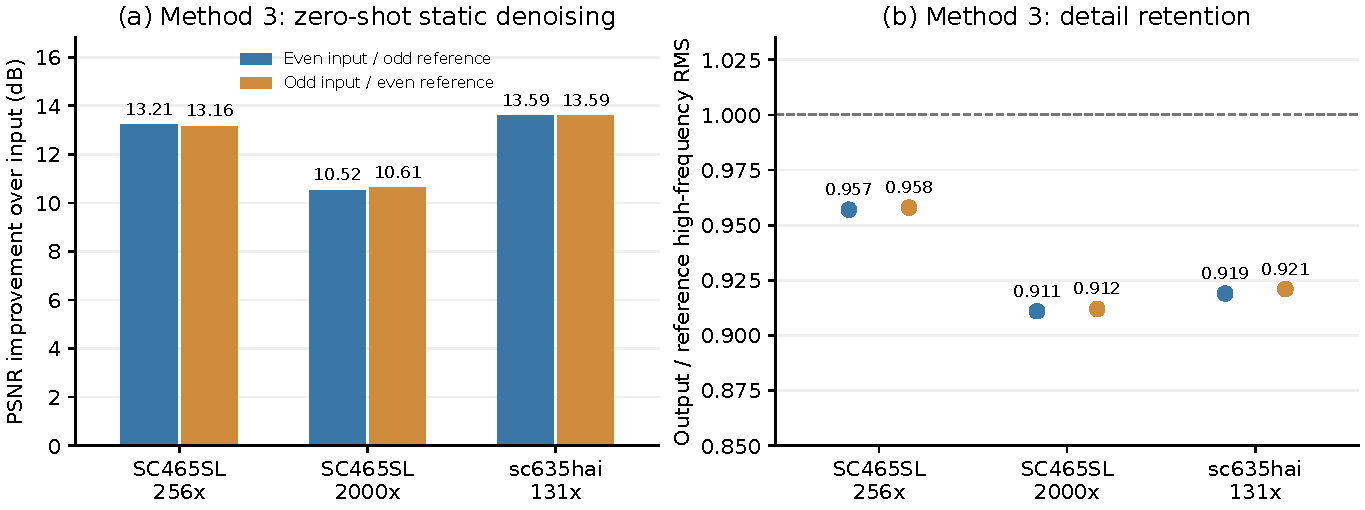
\includegraphics[width=0.78\textwidth]{generalization_static.pdf}
\caption{方法3在三组未参与训练的目标域静态数据上的泛化，左边是相对输入的 PSNR 提升，右边是高频保持率。数据来自表\ref{tab:zero_shot}，参考都取互斥奇偶帧池。}
\label{fig:zero_shot_plot}
\end{figure}

sc635hai 131x 是在低色温、蓝通道白平衡补偿幅度较大的条件下拍的，方法3在这里的静态去噪能力依然很强。图\ref{fig:sc635_static}给出输入、方法3和相反奇偶池的静态参考，背景卡片和人偶的结构都还在。表\ref{tab:zero_shot}是方法3的零样本结果；后面用131x 训专用头得到的数字单独放在第\ref{sec:head_results}节，两个实验不混着看。

\begin{figure}[H]
\centering
\makebox[0.32\textwidth]{输入}\hfill\makebox[0.32\textwidth]{方法3（零样本）}\hfill\makebox[0.32\textwidth]{相反奇偶池参考}\\[0.25em]
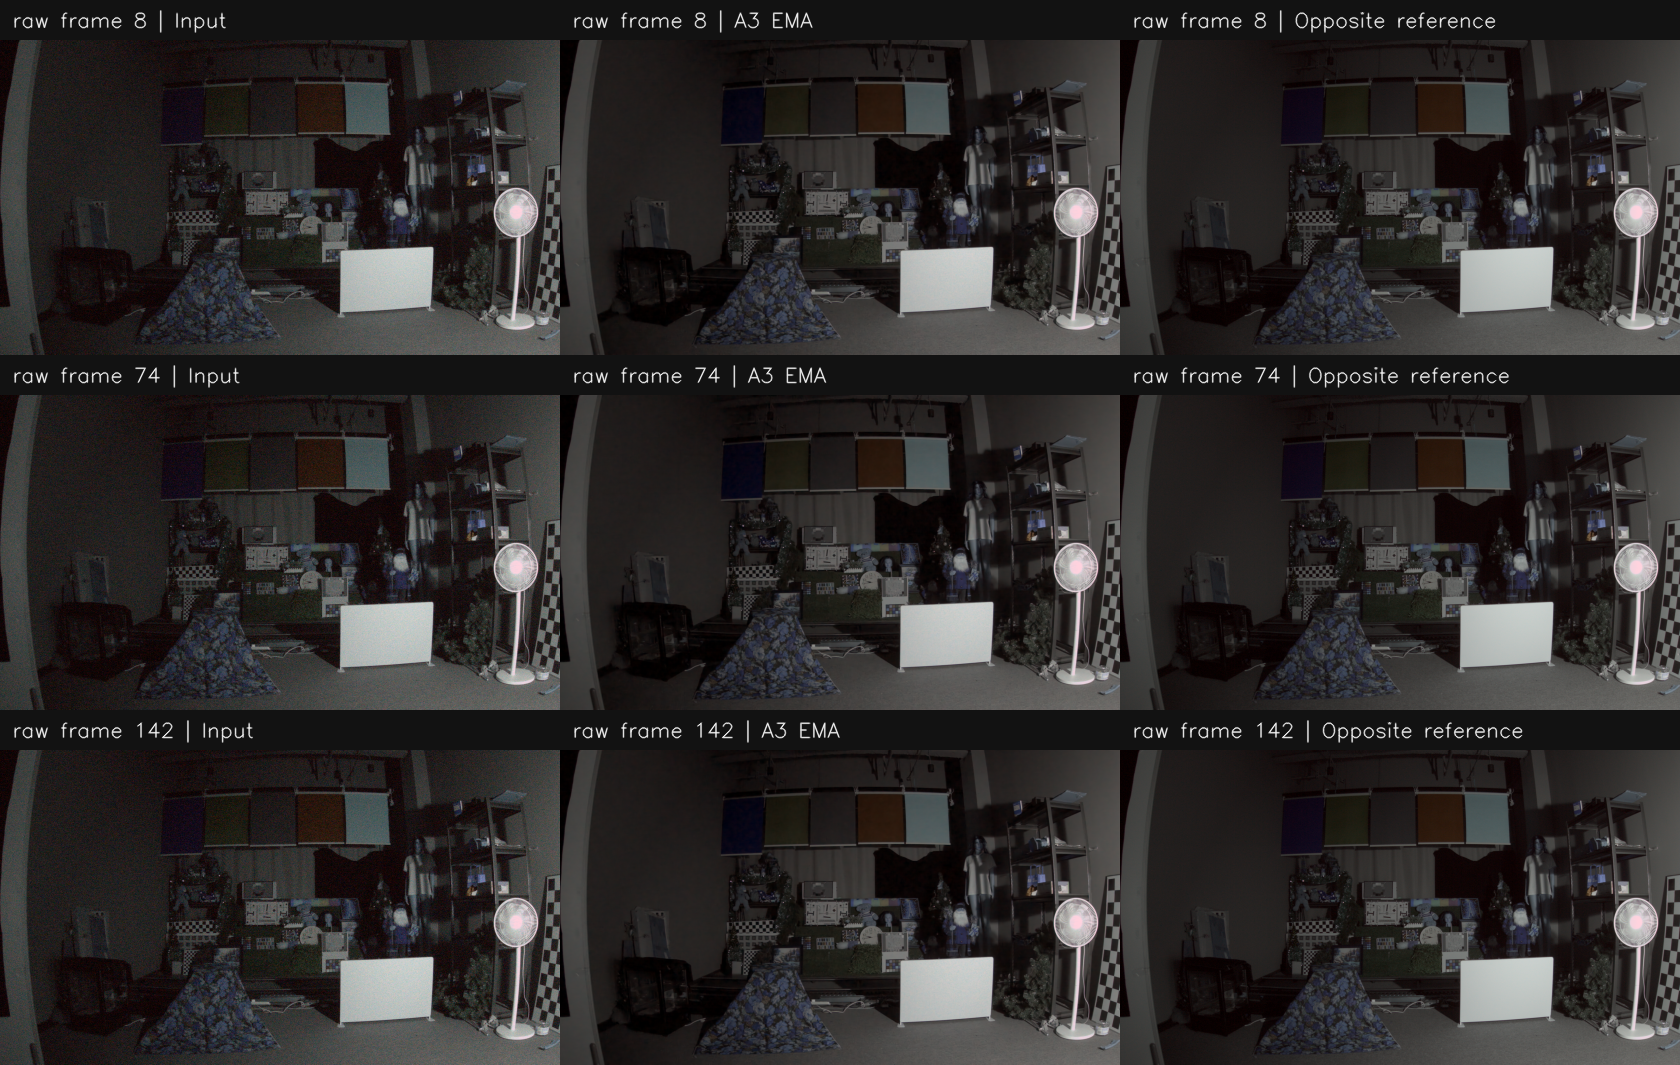
\includegraphics[width=\textwidth,trim=0 710 0 40,clip]{generalization_sc635hai_131x.png}
\caption{sc635hai 131x 低色温数据的零样本静态对比，取偶输入方向的第8帧。参考是对侧奇数帧池的静态均值，动态像素不计入静态指标。}
\label{fig:sc635_static}
\end{figure}

\subsection{sc635hai专用输出头：适配域与动态保留集}
\label{sec:head_results}

方法8在131x 上的指标来自训练数据尾段复评，这一段参与过训练采样，不能算独立泛化结果。表\ref{tab:head_results}里，专用头在静态域只带来约0.034\db{}的变化，高频和时序指标基本没动。16x 动态保留集没有参加训练；因为没有干净的动态目标，这里只报诊断量。

\begin{table}[!htbp]
\centering\small
\caption{sc635hai 专用头的效果。131x 是训练数据尾段复评，16x 是完整保留的动态序列；本表和零样本表用的评测样本不同，基线数值不能混用。}
\label{tab:head_results}
\begin{tabular}{llrr}
\toprule
数据与协议 & 指标 & 方法3 & 方法8专用头 \\
\midrule
131x适配域 & 静态PSNR，偶方向(dB) & 52.3535 & 52.3875 \\
 & 静态PSNR，奇方向(dB) & 52.3552 & 52.3884 \\
 & HF比（约） & 0.9199 & 0.9181 \\
 & temporal MAD(DN) & 2.1628 & 2.1247 \\
\midrule
16x动态保留集 & HF诊断比 & 0.763605 & 0.763078 \\
 & motion/input ratio & 0.599602 & 0.596438 \\
 & temporal MAD(DN) & 14.6745 & 14.6218 \\
 & 端点裁剪 & 2.1994\% & 1.9344\% \\
 & legal RAW fraction & 100\% & 100\% \\
\bottomrule
\end{tabular}
\end{table}

\begin{figure}[!htbp]
\centering\triplehead
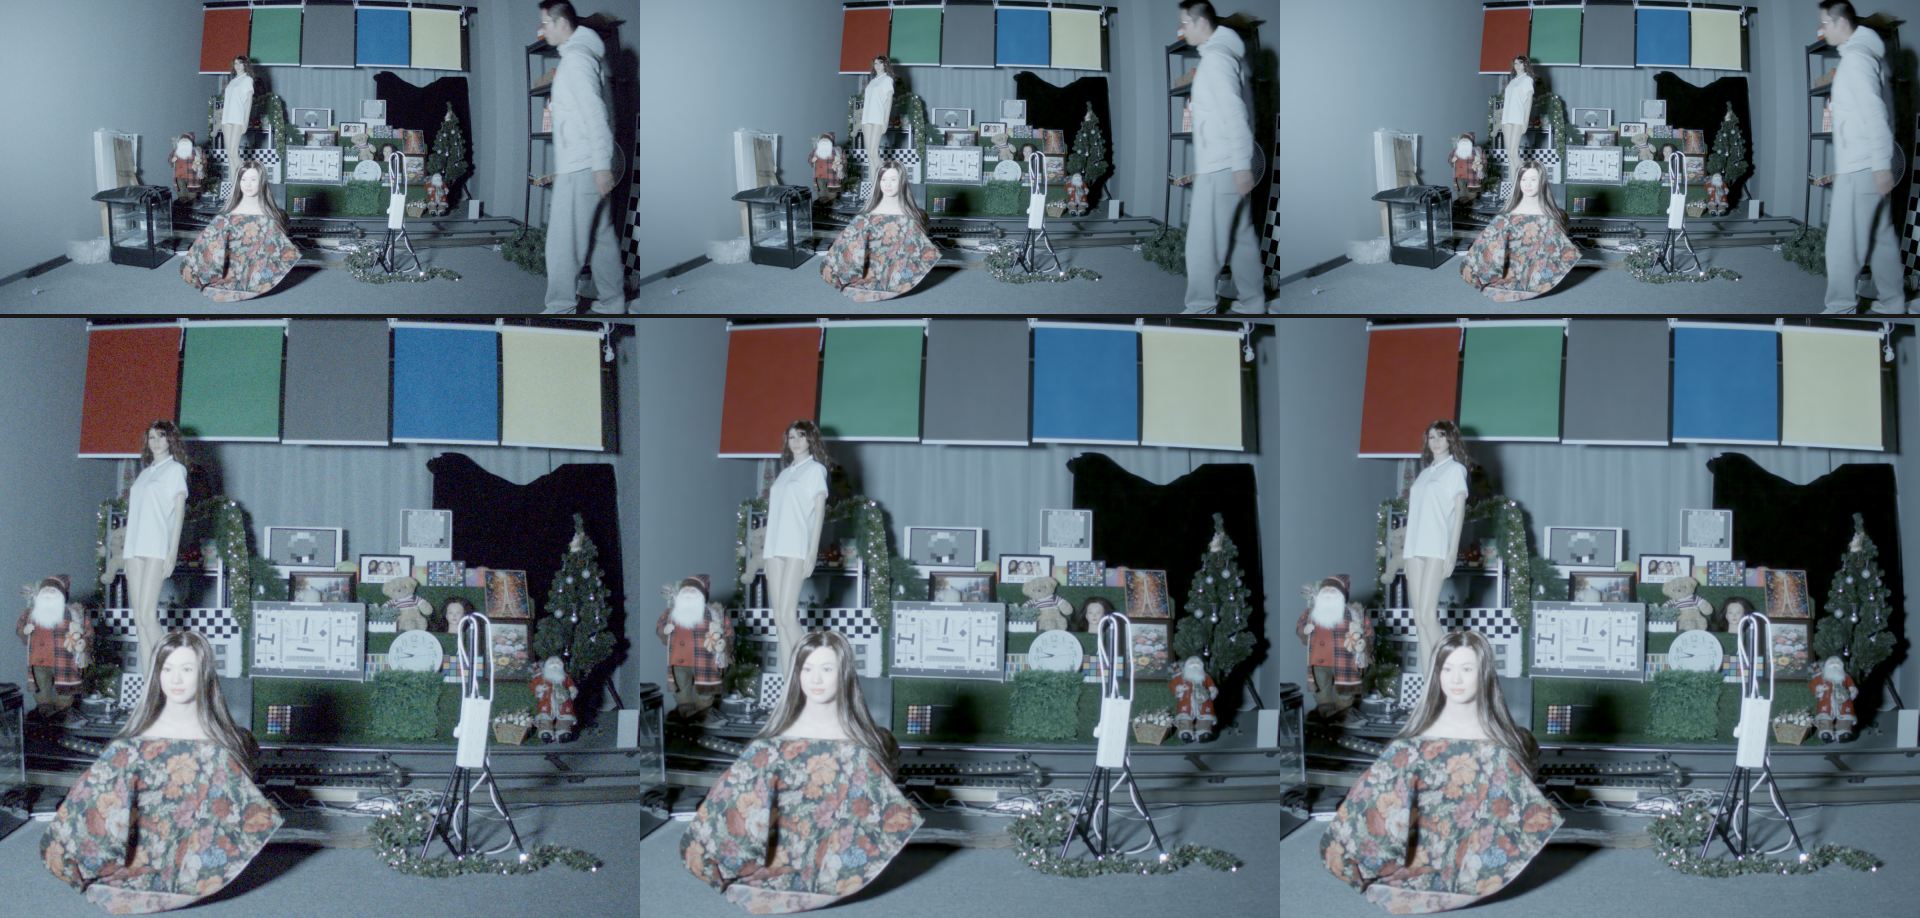
\includegraphics[width=\textwidth]{fig16_sc635hai_traditional_isp.png}
\caption{sc635hai 16x 动态保留集：输入、方法3、方法8专用输出头。上为全景，下为同位置局部；两种输出在结构和纹理上很接近。}
\label{fig:sc635_head}
\end{figure}

图\ref{fig:sc635_head}里，方法8的变化基本集中在输出映射上，动态结构上看不出可辨的提升，所以它仍然只是“sc635hai 专用可选头”。跨传感器静态泛化的主要证据，还是没做任何目标域适配的方法3。

\subsection{室外、高增益和sc450ai数据集的实际输出}

多数据集展示里也有强噪声、快速运动和复杂纹理。MIS20S1 室外1500x 和训练用的暗房在场景、噪声上都不同。图\ref{fig:outdoor}里方法3把彩噪压下去了，但人物局部出现了姿态平均，树木纹理偏软。这条序列没有干净的动态参考，所以不给动态 PSNR。

\begin{figure}[!htbp]
\centering
\begin{minipage}{0.85\textwidth}
\centering\pairhead
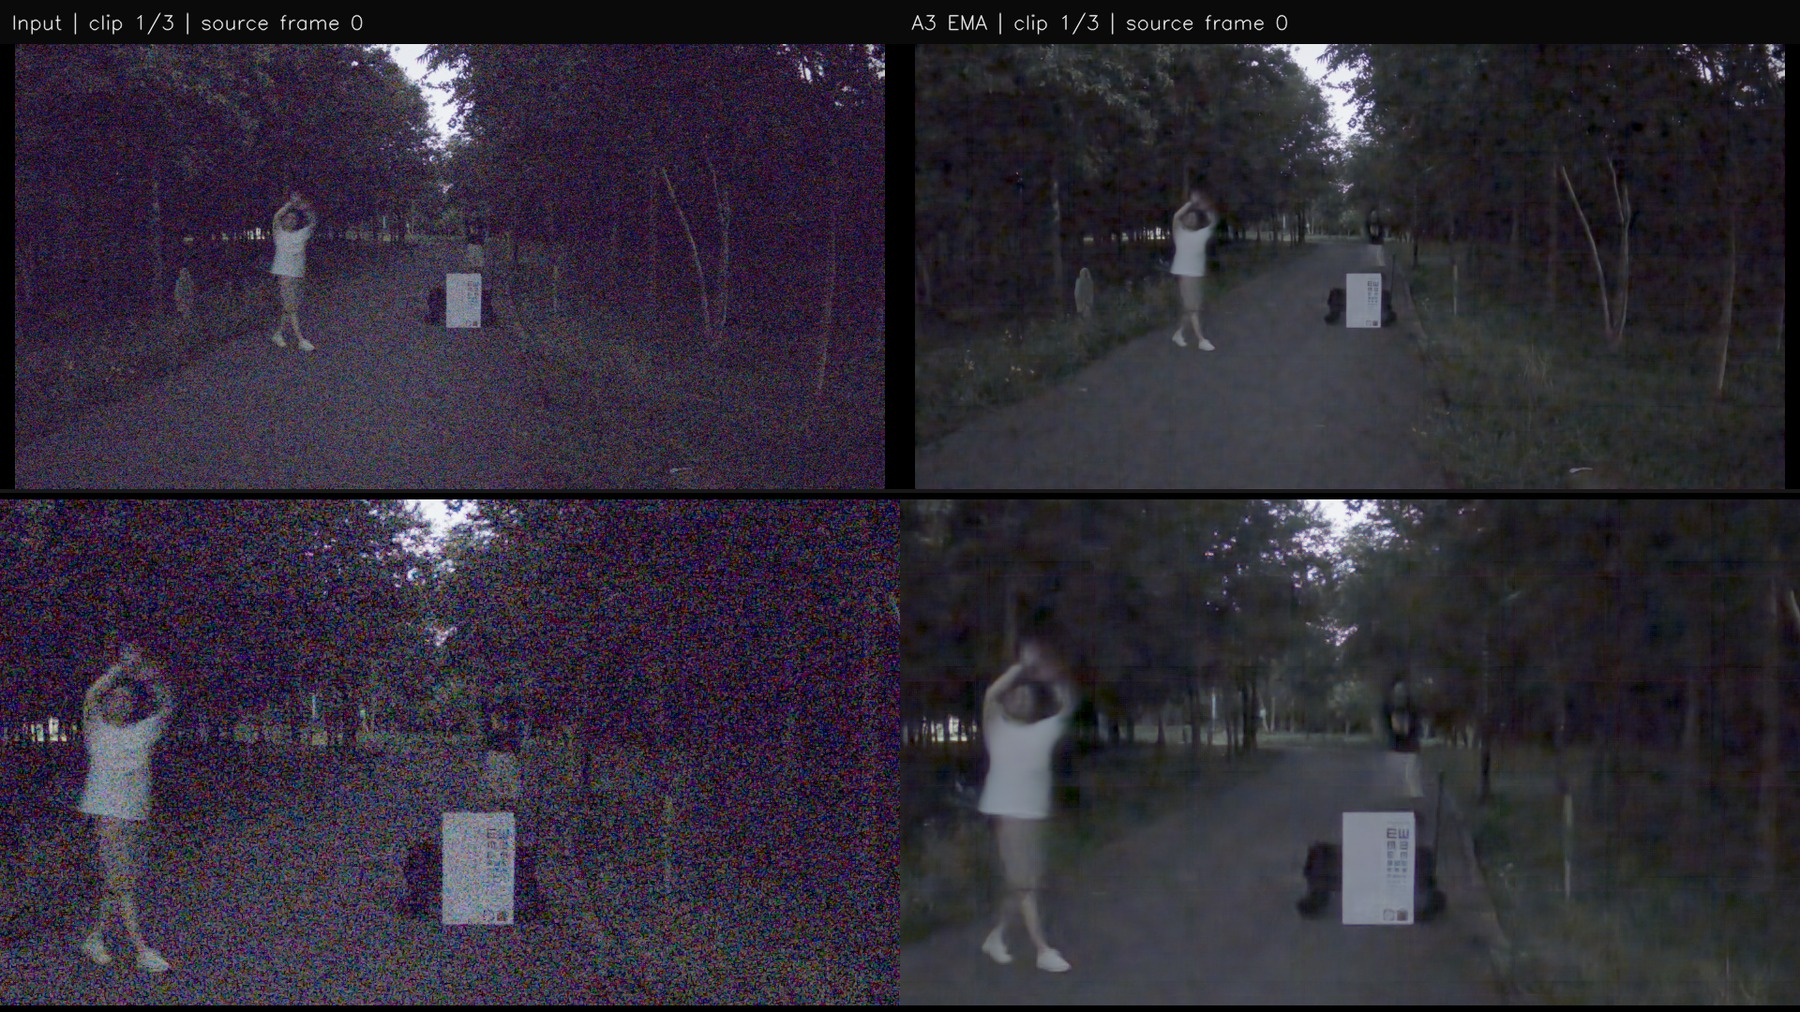
\includegraphics[width=\textwidth,trim=0 0 0 44,clip]{fig15_a3_1500x_isp.jpg}
\end{minipage}
\caption{MIS20S1 室外1500x 的跨场景输出，上为全景，下为中心裁剪。同一份默认权重降噪明显，人物和背景的平滑也看得出来。}
\label{fig:outdoor}
\end{figure}

sc450ai 1435x 黑物运动的零样本诊断里，高频比0.127，端点裁剪约3.28\%，运动/静态时序比0.057/0.088。图\ref{fig:sc450}是方法3的原样输出：黑衣内部结构偏空，边界偏软。804x 灯光变化的高频比0.690，暗部还留着低频色斑。SC465SL 的 difficultpattern 视频里能看到拖影和重影。这些画面和前面三组静态定量合在一起，就是多数据集展示的全貌。

\begin{figure}[!htbp]
\centering
\begin{minipage}{0.85\textwidth}
\centering\pairhead
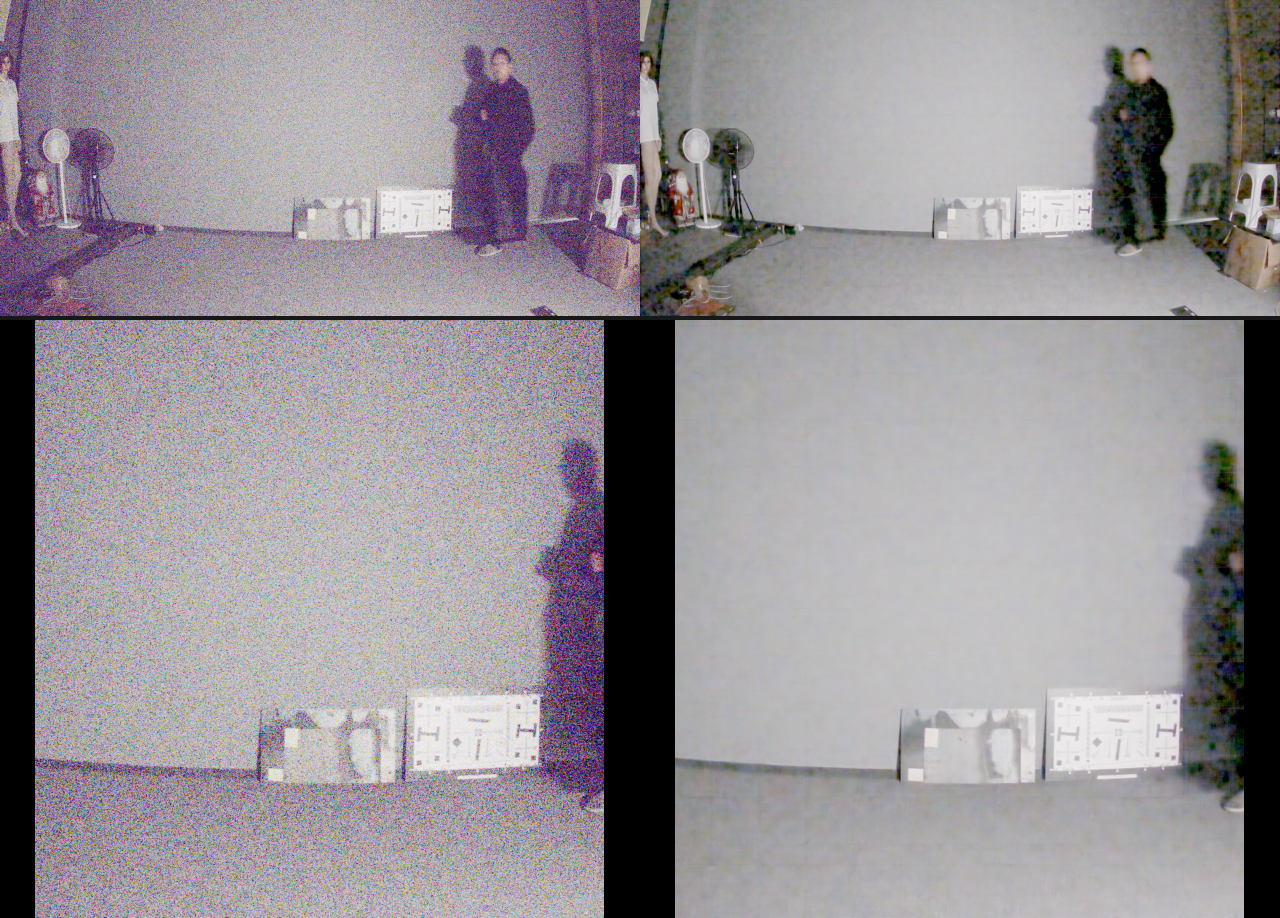
\includegraphics[width=\textwidth]{fig18_sc450ai_traditional_isp.png}
\end{minipage}
\caption{sc450ai 1435x 黑物运动的零样本结果：输入和方法3。黑衣内部和运动轮廓还是偏软。}
\label{fig:sc450}
\end{figure}

\FloatBarrier
表\ref{tab:result_scope}汇总上述数据集的评测协议与实际观察。

{\small
\begin{longtable}{P{0.26\textwidth}P{0.23\textwidth}P{0.40\textwidth}}
\caption{最终方法在不同公司数据集中的展示结果。}\label{tab:result_scope}\\
\toprule
数据条件 & 使用权重与协议 & 已观察结果 \\
\midrule
\endfirsthead
\toprule
数据条件 & 使用权重与协议 & 已观察结果（续） \\
\midrule
\endhead
\bottomrule
\endfoot
MIS20S1暗房645x & 方法3；训练覆盖域、跨增益参考 & +5.22\db，HF 0.971 \\
MIS20S1暗房1000x & 方法3；真实增益留出、原生参考 & +8.65\db；互斥奇偶验证53.10/53.07\db \\
SC465SL暗室256x/2000x & 方法3；跨传感器零样本静态 & +10.52--13.21\db，HF 0.911--0.958 \\
sc635hai低色温131x & 方法3；跨传感器零样本静态 & 约+13.59\db，HF 0.919--0.921 \\
sc635hai动态16x & 方法3及方法8专用头；动态保留集 & 两者画面接近；专用头未见明显新增伪影 \\
MIS20S1室外1500x & 方法3；跨场景动态观察 & 噪声下降，人物姿态与树木结构偏平滑 \\
sc450ai、复杂纹理动态 & 方法3；零样本压力测试 & 可见结构平滑、色斑或重影，不计为通过的静态泛化结果 \\
\end{longtable}
}

\FloatBarrier

\begin{thebibliography}{99}
%========================================================

\bibitem{r1} H. Yue, C. Cao, L. Liao, R. Chu, and J. Yang. Supervised Raw Video Denoising With a Benchmark Dataset on Dynamic Scenes. In \emph{Proceedings of the IEEE/CVF Conference on Computer Vision and Pattern Recognition (CVPR)}, pp. 2301--2310, 2020.

\bibitem{r3} J. Liang, Y. Fan, X. Xiang, R. Ranjan, E. Ilg, S. Green, J. Cao, K. Zhang, R. Timofte, and L. Van Gool. Recurrent Video Restoration Transformer with Guided Deformable Attention. In \emph{Advances in Neural Information Processing Systems (NeurIPS)}, 2022.

\bibitem{r4} J. Lehtinen, J. Munkberg, J. Hasselgren, S. Laine, T. Karras, M. Aittala, and T. Aila. Noise2Noise: Learning Image Restoration without Clean Data. In \emph{Proceedings of the International Conference on Machine Learning (ICML)}, PMLR 80:2965--2974, 2018.

\bibitem{r5} A. Krull, T.-O. Buchholz, and F. Jug. Noise2Void -- Learning Denoising from Single Noisy Images. In \emph{Proceedings of the IEEE/CVF Conference on Computer Vision and Pattern Recognition (CVPR)}, pp. 2129--2137, 2019.

\bibitem{r6} J. Batson and L. Royer. Noise2Self: Blind Denoising by Self-Supervision. In \emph{Proceedings of the International Conference on Machine Learning (ICML)}, PMLR 97:524--533, 2019.

\bibitem{r7} A. Foi, M. Trimeche, V. Katkovnik, and K. Egiazarian. Practical Poissonian-Gaussian Noise Modeling and Fitting for Single-Image Raw-Data. \emph{IEEE Transactions on Image Processing}, 17(10):1737--1754, 2008.

\bibitem{r8} T. Brooks, B. Mildenhall, J. T. Barron, J. Chen, D. Sharlet, and R. Ng. Unprocessing Images for Learned Raw Denoising. In \emph{Proceedings of the IEEE/CVF Conference on Computer Vision and Pattern Recognition (CVPR)}, pp. 11036--11045, 2019.

\bibitem{r9} C. Godard, K. Matzen, and M. Uyttendaele. Deep Burst Denoising. In \emph{Proceedings of the European Conference on Computer Vision (ECCV)}, 2018.

\bibitem{r10} S. W. Hasinoff, D. Sharlet, R. Geiss, A. Adams, J. T. Barron, F. Kainz, J. Chen, and M. Levoy. Burst Photography for High Dynamic Range and Low-Light Imaging on Mobile Cameras. \emph{ACM Transactions on Graphics}, 35(6):192, 2016.

\bibitem{r11} T. Kroeger, R. Timofte, D. Dai, and L. Van Gool. Fast Optical Flow Using Dense Inverse Search. In \emph{Proceedings of the European Conference on Computer Vision (ECCV)}, pp. 471--488, 2016.

\bibitem{r12} E. Reinhard, M. Stark, P. Shirley, and J. Ferwerda. Photographic Tone Reproduction for Digital Images. \emph{ACM Transactions on Graphics}, 21(3):267--276, 2002.

\bibitem{r13} P. Charbonnier, L. Blanc-Feraud, G. Aubert, and M. Barlaud. Two Deterministic Half-Quadratic Regularization Algorithms for Computed Imaging. In \emph{Proceedings of the IEEE International Conference on Image Processing (ICIP)}, vol. 2, pp. 168--172, 1994.

\bibitem{r14} K. Zhang, W. Zuo, Y. Chen, D. Meng, and L. Zhang. Beyond a Gaussian Denoiser: Residual Learning of Deep CNN for Image Denoising. \emph{IEEE Transactions on Image Processing}, 26(7):3142--3155, 2017.

\bibitem{r15} D. Maggioni, E. Sanchez-Monge, and A. Foi. Efficient Multi-Stage Video Denoising With Recurrent Spatio-Temporal Fusion. In \emph{Proceedings of the IEEE/CVF Conference on Computer Vision and Pattern Recognition (CVPR)}, 2021.

\bibitem{r16} M. Tassano, J. Delon, and T. Veit. FastDVDNet: Towards Real-Time Deep Video Denoising Without Flow Estimation. In \emph{Proceedings of the IEEE/CVF Conference on Computer Vision and Pattern Recognition (CVPR)}, 2020.

\bibitem{r17} B. Mildenhall, J. T. Barron, J. Chen, D. Sharlet, R. Ng, and R. Carroll. Burst Denoising with Kernel Prediction Networks. In \emph{Proceedings of the IEEE/CVF Conference on Computer Vision and Pattern Recognition (CVPR)}, 2018.

\bibitem{r18} A. Buades, B. Coll, and J.-M. Morel. A Non-Local Algorithm for Image Denoising. In \emph{Proceedings of the IEEE/CVF Conference on Computer Vision and Pattern Recognition (CVPR)}, 2005.

\bibitem{r19} K. Dabov, A. Foi, V. Katkovnik, and K. Egiazarian. Image Denoising by Sparse 3-D Transform-Domain Collaborative Filtering. \emph{IEEE Transactions on Image Processing}, 16(8):2080--2095, 2007.

\bibitem{r20} S. Guo, Z. Yan, K. Zhang, L. Zhang, and W. Zuo. Toward Convolutional Blind Denoising of Real Photographs. In \emph{Proceedings of the IEEE/CVF Conference on Computer Vision and Pattern Recognition (CVPR)}, 2019.

\end{thebibliography}

\FloatBarrier
\appendix
\section{采纳方法的超参数与模型配置}
\label{app:configuration}

附录记的是方法3和方法8那个 sc635hai 专用可选头的最终配置。训练设置以最终 checkpoint 里保存的配置和优化器状态为准，模型和损失按对应实现核对，展示视频的编码按实际产物记录。下面的文件与目录均链接到 GitHub 仓库，显示路径相对该项目在仓库中的根目录；未收录的材料单独注明。

\subsection{权重与运行环境}

\begin{description}\raggedright
\item[GitHub项目目录] \url{https://github.com/JingZe-Liang/SigmaStar_AIISP/tree/main/Stage2/9_19-10_1/Task3/XWJ/RECOVERED_Stage2_DenoiseModel_20261010}
\item[Python环境] Python 3.12，环境名 \texttt{aaa\_312}；运行时使用该环境中的 \texttt{python}。
\item[方法3最终权重] \texttt{checkpoint\_step\_005000.pth}，大小约156.33 MiB，超过本次普通 Git 上传的单文件限制，未收录到仓库；训练配置与日志见 \repodir{artifacts/finetune_mis20s1/training/}。使用该权重时读取 \texttt{ema} 字段。
\item[方法3 SHA-256] {\small\path{97c4332f685f98959b243e4b100434469f714aed6329e100d22b6d8552592e0b}}
\item[方法8专用权重] \repofile{artifacts/a8_sensor_adaptation/sc635hai/training_20261013/checkpoint_step_000500.pth}，读取 \texttt{ema} 字段。
\item[方法8 SHA-256] {\small\path{8e4980a43767b5b83ecc064e8cdce2f685ea452e94af48a1f4ca252004765b3f}}
\end{description}

\subsection{方法3训练超参数}

\begin{longtable}{P{0.27\textwidth}P{0.65\textwidth}}
\caption{最终主方法的训练与采样配置。}\label{tab:training_config}\\
\toprule 项目 & 实际设置 \\ \midrule
\endfirsthead
\toprule 项目 & 实际设置（续） \\ \midrule
\endhead
\bottomrule\endfoot
初始化 & 公开 CRVD 预训练权重 \repofile{artifacts/pretrained/STaR-RAW-L_CRVD.pth}，strict加载 \\
可训练范围 & 全模型，共7,505,716个参数、1208个参数张量 \\
总优化步数 & 5000；从step 200恢复至step 5000 \\
训练batch size & 1；每次优化包含1个8帧样本 \\
学习率 & 固定 $1\times10^{-4}$，无学习率调度器 \\
优化器 & Adam，$\beta_1=0.9$、$\beta_2=0.999$、$\epsilon=10^{-8}$ \\
优化器其他项 & weight decay为0，amsgrad为False \\
数值精度 & FP32；无autocast、GradScaler或梯度累积 \\
梯度裁剪 & 未使用 \\
EMA & decay=0.999，每次optimizer step后更新参数，buffer直接复制；推理读取EMA \\
随机种子 & 20260921；设置Python、NumPy、PyTorch和CUDA随机种子 \\
输入/输出 & $(B,T,C,H,W)=(1,8,4,64,64)$，输出对应8帧 \\
真实:合成比例 & 配置0.5:0.5；512项采样序列的前256项为真实、后256项为合成 \\
真实训练序列 & MIS20S1暗房128x、313x、632x、645x；不含1000x真实序列 \\
真实时间采样 & 随机起点的连续8帧，frame stride=1 \\
合成时间采样 & 每个增益8个噪声变体，从变体池循环取8帧，干净内容相同 \\
裁剪与增强 & 随机 $64\times64$ packed裁剪、真实时窗、合成噪声；未加入翻转或旋转 \\
样本随机状态 & 索引 $i$ 使用 \texttt{seed + i * 104729}；合成变体使用 \texttt{seed + record\_index * 1009 + variant} \\
DataLoader & 默认512项，shuffle=False，num\_workers=0，drop\_last=True；耗尽后重新遍历 \\
训练输出裁剪 & 预测先clamp到 $[0,1]$，再计算损失 \\
最终权重选择 & step-5000 EMA；未将后续运动、统一后训练或门控候选合并进去 \\
\end{longtable}

实际用的配置文件是 \repofile{artifacts/finetune_mis20s1/training/a3_config.json}，训练和采样实现在 \repofile{src/raw_fusion/finetune/a3.py}。

\subsection{参考、归一化与损失设置}

\begin{longtable}{P{0.27\textwidth}P{0.65\textwidth}}
\caption{主方法监督与损失参数。}\label{tab:loss_config}\\
\toprule 项目 & 设置 \\ \midrule
\endfirsthead
\toprule 项目 & 设置（续） \\ \midrule
\endhead
\bottomrule\endfoot
主参考 & MIS20S1暗房10x的200帧；packed形状 $(4,540,960)$ \\
通道顺序 & R、Gr、Gb、B \\
主参考黑电平 & R=266.125、Gr=275.625、Gb=275.375、B=267.0\dn \\
白电平 & 4095\dn \\
真实输入映射 & 按每条流manifest中的整数位移配准；逐通道slope/intercept映射到参考域，再按式\eqref{eq:normalization}归一化 \\
有效掩码 & 参考有效区 $\cap$ 8帧均静态 $\cap$ 全部8帧/4通道均未饱和；合成样本不另加运动掩码 \\
饱和阈值 & 映射参考域3800\dn，归一化阈值按各参考通道黑电平换算 \\
运动阈值 & 对应采样位置的运动mask $<0.5$，全部8帧同时满足 \\
损失总式 & $\mathcal L_{\mathrm{char}}+0.1\mathcal L_{\mathrm{grad}}+0.1\mathcal L_{\mathrm{hp}}$ \\
Charbonnier & $\sqrt{(\hat y-y)^2+10^{-6}}$；标准 $\epsilon^2$ 记法下 $\epsilon=10^{-3}$ \\
梯度损失 & 水平、垂直梯度幅值差的masked L1，两方向各0.5；相邻mask相乘 \\
高通损失 & $H(u)=u-\mathrm{AvgPool3d}(u)$ 后的masked L1 \\
高通池化 & kernel=$(1,3,3)$，stride=1，padding=$(0,1,1)$；默认零填充且包含填充计数 \\
掩码归约 & 掩码沿通道展开；分母为mask.sum().clamp\_min(1)，逐有效元素平均 \\
动态损失/教师蒸馏 & 最终方法3未使用 \\
\end{longtable}

参考的统计和空间资源分别见 \repofile{artifacts/finetune_mis20s1/supervision/references/a1_reference_report.json} 和同目录的 \repofile{artifacts/finetune_mis20s1/supervision/references/a1_reference_manifest.json}。配准、曝光系数和运动掩码是逐流记在 \repodir{artifacts/finetune_mis20s1/supervision/stream_manifests/} 里的，没有用一组曝光系数打发所有流。

\subsection{网络构造参数}

\begin{longtable}{P{0.31\textwidth}P{0.61\textwidth}}
\caption{STaR-RAW时空恢复主干的实际构造配置。}\label{tab:model_config}\\
\toprule 参数 & 设置 \\ \midrule
\endfirsthead
\toprule 参数 & 设置（续） \\ \midrule
\endhead
\bottomrule\endfoot
输入/输出通道 & 4 / 4 \\
\texttt{upscale} & 1 \\
\texttt{img\_size} & [8, 64, 64] \\
\texttt{window\_size} & [6, 8, 8] \\
\texttt{depths} & [4, 4, 4, 4, 4, 4, 4, 2, 2, 2, 2] \\
\texttt{embed\_dims} & [84, 84, 84, 84, 84, 84, 84, 108, 108, 108, 108] \\
\texttt{num\_heads} & [6, 6, 6, 6, 6, 6, 6, 6, 6, 6, 6] \\
\texttt{indep\_reconsts} & [11, 12]，按构造实参记录 \\
\texttt{mul\_attn\_ratio} & 0.75 \\
\texttt{mlp\_ratio} & 2 \\
\texttt{qkv\_bias / qk\_scale} & True / None \\
\texttt{drop\_path\_rate} & 0.2（配置最大值） \\
归一化 & LayerNorm \\
\texttt{pa\_frames} & 2 \\
\texttt{deformable\_groups} & 12 \\
\texttt{spynet\_path} & None \\
\texttt{recal\_all\_flows} & False \\
\texttt{nonblind\_denoising} & False \\
激活检查点构造参数 & \texttt{use\_checkpoint\_attn=False}，\texttt{use\_checkpoint\_ffn=False}；\texttt{no\_checkpoint\_attn\_blocks} 和 \texttt{no\_checkpoint\_ffn\_blocks} 均为空列表 \\
前7级空间尺度 & [1, 2, 4, 8, 4, 2, 1]；先降采样再恢复 \\
参数与buffer & 参数7,505,716个；buffer 57个，共2,668,800个元素 \\
状态字典 & 每套model/EMA共1265张量，其中1208个为参数张量；张量个数不等于参数量 \\
\end{longtable}

模型配置的入口是 \repofile{src/raw_fusion/finetune/a3.py}，结构实现见 \repofile{src/raw_fusion/finetune/STaR_RAW_arch.py}。

\subsection{噪声合成参数}

表\ref{tab:shot}和表\ref{tab:read}是实际生成器用的逐档经验参数。增益标签 $g$ 对应的 $G$ 等于标签除以100；shot 系数里已经含了这一档的增益，在式\eqref{eq:synthetic}里不要再乘一次 $G$。表里的数保留6位小数，要精确复现就直接读原 JSON 的完整精度。

\begin{table}[!htbp]
\centering\small
\caption{逐增益经验shot系数 $\alpha_{c,g}$，单位DN。}
\label{tab:shot}
\begin{tabular}{rrrrrr}
\toprule
增益标签 & $G$ & R & Gr & Gb & B \\
\midrule
100 & 1 & 0.146240 & 0.133124 & 0.134059 & 0.153964 \\
200 & 2 & 0.303604 & 0.262204 & 0.263975 & 0.301672 \\
400 & 4 & 0.595802 & 0.525547 & 0.529092 & 0.569351 \\
800 & 8 & 1.234060 & 1.038338 & 1.045279 & 1.185013 \\
1600 & 16 & 2.553175 & 2.271041 & 2.286595 & 2.535520 \\
3200 & 32 & 5.057363 & 4.411844 & 4.442612 & 4.909565 \\
6400 & 64 & 10.160087 & 8.932881 & 8.913312 & 10.015178 \\
12800 & 128 & 24.593596 & 24.830152 & 24.722971 & 25.129168 \\
25600 & 256 & 48.717270 & 50.454506 & 50.209071 & 50.189296 \\
\bottomrule
\end{tabular}
\end{table}

\begin{table}[!htbp]
\centering\small
\caption{逐增益read variance $v_{c,g}$，单位DN$^2$。}
\label{tab:read}
\begin{tabular}{rrrrrr}
\toprule
增益标签 & $G$ & R & Gr & Gb & B \\
\midrule
100 & 1 & 1.582505 & 1.582505 & 1.582505 & 1.582505 \\
200 & 2 & 2.813700 & 2.813700 & 2.813700 & 2.813700 \\
400 & 4 & 8.617427 & 8.616957 & 8.616957 & 8.617427 \\
800 & 8 & 29.718838 & 29.718838 & 29.718838 & 29.718838 \\
1600 & 16 & 4.396071 & 4.396071 & 4.396071 & 4.396071 \\
3200 & 32 & 11.254265 & 11.254265 & 11.254265 & 11.254265 \\
6400 & 64 & 39.564642 & 34.466890 & 34.466890 & 34.467829 \\
12800 & 128 & 114.346263 & 114.346263 & 114.346263 & 114.346263 \\
25600 & 256 & 364.052709 & 364.046605 & 364.049657 & 364.049657 \\
\bottomrule
\end{tabular}
\end{table}

生成器使用的聚合通道相关矩阵为
\begin{equation}
C=\begin{bmatrix}
1 & 0.01588756 & 0.00647320 & 0.00093781\\
0.01588756 & 1 & 0.00753526 & 0.00049242\\
0.00647320 & 0.00753526 & 1 & 0.02030878\\
0.00093781 & 0.00049242 & 0.02030878 & 1
\end{bmatrix}.
\end{equation}
固定图样偏置从主参考 manifest 的 \texttt{fpn\_paths.offset\_dn} 空间数组里读。每档8个噪声变体各用独立随机数，先 round 到1\dn{}格点、再 clip 到 $[0,4095]$，存成 uint16。完整的噪声模型在 \repofile{artifacts/finetune_mis20s1/noise_model/noise_model.json}，生成器是 \repofile{src/raw_fusion/finetune/noise.py} 里的 \texttt{generate\_noisy\_frame}。

\subsection{推理、评测与固定 ISP 参数}

\begin{longtable}{P{0.27\textwidth}P{0.65\textwidth}}
\caption{最终主方法的推理与展示配置。}\label{tab:inference_config}\\
\toprule 项目 & 设置 \\ \midrule
\endfirsthead
\toprule 项目 & 设置（续） \\ \midrule
\endhead
\bottomrule\endfoot
模型状态 & EMA，eval模式；不更新参数 \\
连续视频时间窗口 & 8帧，窗口步长4；不足8帧时重复末帧，丢弃补齐位置的输出 \\
空间tile/步长 & $64\times64$ packed / 56 packed；完整画面覆盖 \\
重叠区域 & 时域和空域均采用等权累计、除以覆盖计数 \\
分块并行批大小 & 全数据集展示使用tile\_batch=12；跨传感器审计入口配置为2，原始全帧评估入口常用8；均不改变训练bs=1 \\
输出裁剪 & 归一化域 $[0,1]$，再按对应管线恢复DN \\
跨传感器静态采样 & 输入与参考奇偶帧池互斥；每片段8帧、原视频stride=2。SC465SL每方向5片段（40帧），sc635hai零样本每方向3片段（24帧），专用头尾段复评每方向1片段（8帧） \\
静态有效区 & 奇偶参考置信度 $\ge0.9$ \\
展示采样 & 每流首、中、尾各1个连续8帧片段，共24帧；45流共1080帧 \\
去马赛克 & canonical Bayer重建，OpenCV edge-aware \\
曝光选择 & 每条流由输入99.5百分位确定；Reinhard后线性目标0.8，EV范围 $[-6,8]$；输入与输出共享冻结值 \\
白平衡 & 各流manifest中的固定WB，输入与输出共享 \\
色调与高光 & Reinhard tone mapping；高光重建开启；随后sRGB gamma \\
其他ISP项 & 2DNR/3DNR关闭，false color suppression关闭 \\
色彩模式 & uncalibrated camera RGB；未使用传感器ColorMatrix \\
实际预览视频 & HEVC（libx265），CRF16，yuv444p，1920$\times$1080，6fps；每视频24帧 \\
面板布局 & 输入左、方法3右；上为全景、下为固定中心裁剪 \\
\end{longtable}

表\ref{tab:inference_config}里的 ISP 和视频项对应45流全数据集预览。图\ref{fig:mis1000}、图\ref{fig:sc635_head}、图\ref{fig:sc450}是把各自评测时缓存的同帧 RAW 用这套传统 ISP 重新渲染的，固定曝光分别是4.7393、2.0011、6.2803 EV，各列共用同一组参数。奇偶参考面板沿用原审计的普通 Bayer 去马赛克和 sRGB 变换；重渲染只改展示，不动 RAW 域指标。

分块实现在 \repofile{src/raw_fusion/finetune/a4.py}；跨传感器清单是 \repofile{configs/a3_cross_sensor_zero_shot_20261012.json} 和 \repofile{configs/a3_cross_sensor_extension_20261012.json}；全数据集设置见 \repofile{configs/a3_all_dataset_traditional_isp_preview_20261017.json}。这份配置里 \texttt{preferred\_encoder} 写的是 libx264，但45个实际视频和对应的 \texttt{video\_manifest.json} 都是 libx265，表\ref{tab:inference_config}按实际产物记。

\subsection{方法8的sc635hai专用头完整配置}

\begin{longtable}{P{0.27\textwidth}P{0.65\textwidth}}
\caption{专用可选输出头的训练设置。}\label{tab:head_config}\\
\toprule 项目 & 实际设置 \\ \midrule
\endfirsthead
\toprule 项目 & 实际设置（续） \\ \midrule
\endhead
\bottomrule\endfoot
初始化与范围 & 方法3 step-5000 EMA；主干冻结且eval，仅训练输出头 \\
可训练模块 & \texttt{norm}、\texttt{conv\_after\_body}、\texttt{conv\_last}，共6张量、12,400参数 \\
头部结构与参数 & LayerNorm108：216；Linear108$\to$84：9156；Conv3d84$\to$4，kernel=$(1,3,3)$：3028 \\
目标传感器样本 & sc635hai 131x低色温，共150帧，完整范围 $[0,150)$ \\
输入/目标帧池 & 偶池0,2,\ldots,148与奇池1,3,\ldots,149互换；每池75帧，目标为对侧静态均值 \\
时间窗口 & 同一池8帧，即原视频frame stride=2 \\
训练batch / 步数 & 1 / 500 \\
随机种子 & 20261013 \\
学习率与优化器 & 固定 $10^{-5}$，Adam，betas=$(0.9,0.999)$，eps=$10^{-8}$，weight decay=0，amsgrad=False；无调度器 \\
精度与损失 & BF16 autocast，损失转FP32；与式\eqref{eq:loss}相同，权重1/0.1/0.1 \\
EMA / 梯度裁剪 & decay=0.999 / gradient norm=1.0 \\
patch与有效区域 & $64\times64$ packed；静态置信度 $\ge0.9$，输入未饱和；有效比例至少0.25，最多尝试32次裁剪 \\
目标域增强 & 水平翻转、垂直翻转、转置，各以0.5概率施加 \\
回放概率与实绩 & MIS20S1回放概率0.5；实际回放262步，sc635hai采样238步；回放沿用主方法数据管线 \\
检查点间隔 & 每100步保存，最终保留step-500 EMA \\
131x静态复评片段 & 偶输入134,136,\ldots,148；奇输入135,137,\ldots,149。该尾段参与训练采样，不作为独立留出 \\
独立动态保留集 & sc635hai 16x运动彩色200帧，不参与训练；仅无参考诊断与固定ISP观察 \\
用途 & sc635hai专用可选头，不替代默认方法3 \\
\end{longtable}

配置文件在 \repofile{configs/a8_sc635hai_adaptation_20261013.json}，训练摘要和保存的配置在 \repodir{artifacts/a8_sensor_adaptation/sc635hai/training_20261013/}，实现在 \repofile{src/raw_fusion/finetune/a8_adaptation.py}。

\subsection{结果来源与复现入口}

主方法的静态评估在 \repodir{artifacts/finetune_mis20s1/evaluation/}，跨传感器静态结果在 \repodir{artifacts/a3_cross_sensor_zero_shot_20261012/} 和 \repodir{artifacts/a3_cross_sensor_extension_20261012/}，45流完整预览在 \repodir{artifacts/a3_all_dataset_traditional_isp_preview_20261017/}。专用输出头的解释和检查结果见 \repofile{docs/A8_SC635HAI_ADAPTATION_RESULT_2026-10-13.md}。文件名都保留原始实验标识，方便对回已有产物。

克隆仓库并进入上述项目目录，准备原始数据及未收录的方法3最终权重后，可执行下面这些纯评测命令，按对应协议复现主要结果。命令里的 \texttt{python} 指本附录记录的那个 Python 环境。

{\small
\begin{verbatim}
python scripts/run_a4_eval.py --max-frames 200 \
  --tile-batch 8 \
  --output-dir artifacts/finetune_mis20s1/evaluation
python scripts/run_native_1000x_eval.py --max-frames 200 \
  --tile-batch 8 \
  --output-dir artifacts/finetune_mis20s1/evaluation/native_1000x
python scripts/evaluate_a3_cross_sensor.py \
  --config configs/a3_cross_sensor_zero_shot_20261012.json \
  --output-dir artifacts/a3_cross_sensor_zero_shot_20261012 \
  --phase all --device cuda:0 --tile-batch 2
python scripts/evaluate_a3_cross_sensor.py \
  --config configs/a3_cross_sensor_extension_20261012.json \
  --output-dir artifacts/a3_cross_sensor_extension_20261012 \
  --phase all --device cuda:0 --tile-batch 2
\end{verbatim}
}

结果表里，645x 是训练覆盖域的复评，1000x 是真实增益留出；零样本跨传感器表只用方法3，sc635hai 专用头的131x 尾段属于训练数据复评。复现时要守住这些数据身份和各自的参考定义。

\section{补充探索的记录与图表来源}
\label{app:djc_sources}

第\ref{sec:djc}节的补充探索对应 GitHub 仓库的 \href{https://github.com/JingZe-Liang/SigmaStar_AIISP/tree/main/Stage2/9_19-10_1/Task3/DJC}{\nolinkurl{Stage2/9_19-10_1/Task3/DJC/}}。该目录中的 \href{https://github.com/JingZe-Liang/SigmaStar_AIISP/blob/main/Stage2/9_19-10_1/Task3/DJC/Report.MD}{\nolinkurl{Report.MD}} 是研究报告入口，方法实现位于其下的 \nolinkurl{ExposureDiffusionNAFNet_DJC_experimental/}。下表只为仓库中实际存在的材料提供链接；原交付包中的完整历史归档、训练运行目录及部分验证记录未收录到当前仓库，不能从这些链接直接取得。
{\linespread{1}\footnotesize\renewcommand{\arraystretch}{1.05}
\begin{longtable}{P{0.20\textwidth}P{0.74\textwidth}}
\caption{ExposureDiffusion路线的主要证据入口。}\label{tab:djc_sources}\\
\toprule
内容 & 对应记录 \\
\midrule
\endfirsthead
\toprule
内容 & 对应记录 \\
\midrule
\endhead
\bottomrule
\endfoot
早期噪声研究 & \djcfile{project/code/noise_model/TWO_SHOTS_CVPR2026.md}、\djcfile{project/code/noise_model/ONE_FRAME_DARK_VALIDATION.md}、\djcfile{project/code/noise_model/PNNP_DECOMPOSITION_COMPARISON.md}、\djcfile{project/code/noise_model/QUANTIZED_LIKELIHOOD.md} 与 \djcfile{project/code/noise_model/STATIC_CONDITIONAL_RESIDUAL.md} \\
多传感器自标定 & 原始标定归档未收录；研究说明见上述 DJC 研究报告入口。 \\
单帧1000步适配 & 原始完成审计与训练运行记录未收录；随附曲线数据见 \repofile{docs/assets/stage2_report_20261023/djc/exposure_validation.csv}。 \\
历史模块试验与解冻 & 完整历史实验、运行记录、评估归档及352项汇总台账未收录；仓库中的报告与随附最小数据不替代完整归档。 \\
最终五帧结构与实际训练 & 实现见 \djcfile{project/code/company_exposure/burst_detail/model.py} 和 \djcfile{project/code/scripts/exposure_output_residual_local.py}；训练曲线数据见 \repofile{docs/assets/stage2_report_20261023/djc/v3_validation.csv}；原始运行目录未收录。 \\
固定与补充验证 & 随附分域数据见 \repofile{docs/assets/stage2_report_20261023/djc/v3_domain_comparison.csv}；完整固定验证 JSON、补充裁块及敏感性台账未收录。 \\
165例图像与权重身份 & 报告选用场景图及来源见 \repofile{docs/assets/stage2_report_20261023/djc/figure_sources.json} 和\repodir{docs/assets/stage2_report_20261023/djc/}；完整165例比较图、推理协议及模型权重未收录。 \\
\end{longtable}
}

早期噪声建模的数值是按上述研究记录转述的。对应的原始噪声拟合 JSON 和 NPZ 未收录到仓库，所以这部分只核对了报告和实现，没有把它们当作新完成的独立验收。后续历史训练的352项汇总指标此前已经和原运行 JSON 逐项比对过；五帧候选的固定验证、补充裁块和图像权重身份此前也都分别核过，但当前仓库未收录这些完整原始记录。读者可从上述链接核查已上传的最小数据与实现。

报告里的五张场景图保持原始 PNG 内容，排版时只裁掉了原来的小字号表头和标签。复制来源、文件哈希和最佳权重身份都存在 \repofile{docs/assets/stage2_report_20261023/djc/figure_sources.json} 里。曲线和分域图是用同目录的 \repofile{docs/assets/stage2_report_20261023/djc/plot_djc_results.py} 基于随附的最小 CSV 重绘的，来源记在 \repofile{docs/assets/stage2_report_20261023/djc/plot_sources.json}。这组图里的公开预训练基线和第\ref{sec:adopted}节后训练出来的方法3，始终当成两份不同的权重处理。

\end{document}
